% Options for packages loaded elsewhere
\PassOptionsToPackage{unicode}{hyperref}
\PassOptionsToPackage{hyphens}{url}
\documentclass[
  canadien,
  11pt,
  letterpaper,
]{article}
\usepackage{xcolor}
\usepackage[margin=0.85in]{geometry}
\usepackage{amsmath,amssymb}
\setcounter{secnumdepth}{-\maxdimen} % remove section numbering
\usepackage{iftex}
\ifPDFTeX
  \usepackage[T1]{fontenc}
  \usepackage[utf8]{inputenc}
  \usepackage{textcomp} % provide euro and other symbols
\else % if luatex or xetex
  \usepackage{unicode-math} % this also loads fontspec
  \defaultfontfeatures{Scale=MatchLowercase}
  \defaultfontfeatures[\rmfamily]{Ligatures=TeX,Scale=1}
\fi
\usepackage{lmodern}
\ifPDFTeX\else
  % xetex/luatex font selection
  \setmainfont[]{Segoe UI}
  \setsansfont[]{Segoe UI}
  \setmonofont[]{Consolas}
\fi
% Use upquote if available, for straight quotes in verbatim environments
\IfFileExists{upquote.sty}{\usepackage{upquote}}{}
\IfFileExists{microtype.sty}{% use microtype if available
  \usepackage[]{microtype}
  \UseMicrotypeSet[protrusion]{basicmath} % disable protrusion for tt fonts
}{}
\makeatletter
\@ifundefined{KOMAClassName}{% if non-KOMA class
  \IfFileExists{parskip.sty}{%
    \usepackage{parskip}
  }{% else
    \setlength{\parindent}{0pt}
    \setlength{\parskip}{6pt plus 2pt minus 1pt}}
}{% if KOMA class
  \KOMAoptions{parskip=half}}
\makeatother
\usepackage{color}
\usepackage{fancyvrb}
\newcommand{\VerbBar}{|}
\newcommand{\VERB}{\Verb[commandchars=\\\{\}]}
\DefineVerbatimEnvironment{Highlighting}{Verbatim}{commandchars=\\\{\}}
% Add ',fontsize=\small' for more characters per line
\newenvironment{Shaded}{}{}
\newcommand{\AlertTok}[1]{\textcolor[rgb]{1.00,0.00,0.00}{\textbf{#1}}}
\newcommand{\AnnotationTok}[1]{\textcolor[rgb]{0.38,0.63,0.69}{\textbf{\textit{#1}}}}
\newcommand{\AttributeTok}[1]{\textcolor[rgb]{0.49,0.56,0.16}{#1}}
\newcommand{\BaseNTok}[1]{\textcolor[rgb]{0.25,0.63,0.44}{#1}}
\newcommand{\BuiltInTok}[1]{\textcolor[rgb]{0.00,0.50,0.00}{#1}}
\newcommand{\CharTok}[1]{\textcolor[rgb]{0.25,0.44,0.63}{#1}}
\newcommand{\CommentTok}[1]{\textcolor[rgb]{0.38,0.63,0.69}{\textit{#1}}}
\newcommand{\CommentVarTok}[1]{\textcolor[rgb]{0.38,0.63,0.69}{\textbf{\textit{#1}}}}
\newcommand{\ConstantTok}[1]{\textcolor[rgb]{0.53,0.00,0.00}{#1}}
\newcommand{\ControlFlowTok}[1]{\textcolor[rgb]{0.00,0.44,0.13}{\textbf{#1}}}
\newcommand{\DataTypeTok}[1]{\textcolor[rgb]{0.56,0.13,0.00}{#1}}
\newcommand{\DecValTok}[1]{\textcolor[rgb]{0.25,0.63,0.44}{#1}}
\newcommand{\DocumentationTok}[1]{\textcolor[rgb]{0.73,0.13,0.13}{\textit{#1}}}
\newcommand{\ErrorTok}[1]{\textcolor[rgb]{1.00,0.00,0.00}{\textbf{#1}}}
\newcommand{\ExtensionTok}[1]{#1}
\newcommand{\FloatTok}[1]{\textcolor[rgb]{0.25,0.63,0.44}{#1}}
\newcommand{\FunctionTok}[1]{\textcolor[rgb]{0.02,0.16,0.49}{#1}}
\newcommand{\ImportTok}[1]{\textcolor[rgb]{0.00,0.50,0.00}{\textbf{#1}}}
\newcommand{\InformationTok}[1]{\textcolor[rgb]{0.38,0.63,0.69}{\textbf{\textit{#1}}}}
\newcommand{\KeywordTok}[1]{\textcolor[rgb]{0.00,0.44,0.13}{\textbf{#1}}}
\newcommand{\NormalTok}[1]{#1}
\newcommand{\OperatorTok}[1]{\textcolor[rgb]{0.40,0.40,0.40}{#1}}
\newcommand{\OtherTok}[1]{\textcolor[rgb]{0.00,0.44,0.13}{#1}}
\newcommand{\PreprocessorTok}[1]{\textcolor[rgb]{0.74,0.48,0.00}{#1}}
\newcommand{\RegionMarkerTok}[1]{#1}
\newcommand{\SpecialCharTok}[1]{\textcolor[rgb]{0.25,0.44,0.63}{#1}}
\newcommand{\SpecialStringTok}[1]{\textcolor[rgb]{0.73,0.40,0.53}{#1}}
\newcommand{\StringTok}[1]{\textcolor[rgb]{0.25,0.44,0.63}{#1}}
\newcommand{\VariableTok}[1]{\textcolor[rgb]{0.10,0.09,0.49}{#1}}
\newcommand{\VerbatimStringTok}[1]{\textcolor[rgb]{0.25,0.44,0.63}{#1}}
\newcommand{\WarningTok}[1]{\textcolor[rgb]{0.38,0.63,0.69}{\textbf{\textit{#1}}}}
\usepackage{longtable,booktabs,array}
\newcounter{none} % for unnumbered tables
\usepackage{calc} % for calculating minipage widths
% Correct order of tables after \paragraph or \subparagraph
\usepackage{etoolbox}
\makeatletter
\patchcmd\longtable{\par}{\if@noskipsec\mbox{}\fi\par}{}{}
\makeatother
% Allow footnotes in longtable head/foot
\IfFileExists{footnotehyper.sty}{\usepackage{footnotehyper}}{\usepackage{footnote}}
\makesavenoteenv{longtable}
\usepackage{graphicx}
\makeatletter
\newsavebox\pandoc@box
\newcommand*\pandocbounded[1]{% scales image to fit in text height/width
  \sbox\pandoc@box{#1}%
  \Gscale@div\@tempa{\textheight}{\dimexpr\ht\pandoc@box+\dp\pandoc@box\relax}%
  \Gscale@div\@tempb{\linewidth}{\wd\pandoc@box}%
  \ifdim\@tempb\p@<\@tempa\p@\let\@tempa\@tempb\fi% select the smaller of both
  \ifdim\@tempa\p@<\p@\scalebox{\@tempa}{\usebox\pandoc@box}%
  \else\usebox{\pandoc@box}%
  \fi%
}
% Set default figure placement to htbp
\def\fps@figure{htbp}
\makeatother
\ifLuaTeX
\usepackage[bidi=basic,shorthands=off]{babel}
\else
\usepackage[bidi=default,shorthands=off]{babel}
\fi
\ifPDFTeX
\else
\babelfont{rm}[]{Segoe UI}
\fi
\ifLuaTeX
  \usepackage{selnolig} % disable illegal ligatures
\fi
\setlength{\emergencystretch}{3em} % prevent overfull lines
\providecommand{\tightlist}{%
  \setlength{\itemsep}{0pt}\setlength{\parskip}{0pt}}
\usepackage{xcolor}
\definecolor{orbitCyan}{HTML}{137DA0}
\definecolor{orbitViolet}{HTML}{6D4AA6}
\definecolor{orbitAmber}{HTML}{AC6A15}
\AtBeginDocument{\hypersetup{colorlinks=true,urlcolor=orbitCyan,linkcolor=orbitViolet}}
\AtBeginDocument{\renewcommand{\contentsname}{Table des matières}}
\renewcommand{\maketitle}{\begin{titlepage}\centering
\vspace*{0.7in}
{\color{orbitAmber}\Huge\bfseries Orbit}\par\vspace{0.25in}
{\LARGE Jouer, comprendre, transmettre}\par\vspace{0.2in}
{\large Les quinze interactions de l’atome, du geste au code}\par\vspace{0.55in}

\includegraphics[width=\textwidth]{figures/landing-final.png}\par\vspace{0.55in}
{\color{orbitViolet}\rule{0.65\textwidth}{0.8pt}}\par\vspace{0.2in}
{\large Jean-Sébastien Beaulieu}\par\vspace{0.1in}
Support pédagogique préparé avec Codex\par\vfill
30 septembre 2026 · version 2.1.6\par
\end{titlepage}}
\usepackage{fvextra}
\DefineVerbatimEnvironment{Highlighting}{Verbatim}{commandchars=\\\{\},breaklines,breakanywhere,fontsize=\footnotesize}
\setlength{\emergencystretch}{3em}
\usepackage{fancyhdr}
\pagestyle{fancy}
\fancyhf{}
\fancyhead[L]{\small Orbit · comprendre et transmettre}
\fancyfoot[R]{\thepage}
\renewcommand{\headrulewidth}{0.3pt}
\usepackage{bookmark}
\IfFileExists{xurl.sty}{\usepackage{xurl}}{} % add URL line breaks if available
\urlstyle{same}
\hypersetup{
  pdftitle={Orbit --- jouer{,} comprendre{,} transmettre},
  pdfauthor={Jean-Sébastien Beaulieu · support préparé avec Codex},
  pdflang={fr-CA},
  hidelinks,
  pdfcreator={LaTeX via pandoc}}

\title{Orbit --- jouer, comprendre, transmettre}
\usepackage{etoolbox}
\makeatletter
\providecommand{\subtitle}[1]{% add subtitle to \maketitle
  \apptocmd{\@title}{\par {\large #1 \par}}{}{}
}
\makeatother
\subtitle{Les quinze interactions de l'atome, du geste au code}
\author{Jean-Sébastien Beaulieu · support préparé avec Codex}
\date{30 septembre 2026 · version 2.1.6 · édition de travail}

\begin{document}
\maketitle

{
\setcounter{tocdepth}{2}
\tableofcontents
}
\section{Avant de commencer}\label{avant-de-commencer}

Ce manuel accompagne la version publique
d'\href{https://orbit.securedme.ca/}{Orbit}. Il sert à apprendre en
manipulant, puis à guider un étudiant dans une expérience comparable. Sa
première partie explique la scène et les quinze jeux. Sa seconde partie
transforme ces mécanismes en activités, avec prédictions, essais et
critères de compréhension. Les corrigés sont séparés des consignes pour
laisser une vraie tentative.

\textbf{Statut : exemplaire de travail pour revue.} Le code a été
inspecté et les comportements couverts par la validation cloud sont
indiqués dans l'annexe. Les réponses de l'étudiant et votre propre
apprentissage restent à documenter. Aucun résultat de jeu ne devient
automatiquement une preuve de maîtrise.

Le nom d'atome désigne notre sculpture interactive. Les orbites, le
vortex, les portails et les traces sont des constructions visuelles.
\textbf{Le site ne calcule pas une simulation quantique.} Les unités de
scène servent à régler l'effet ; elles ne sont pas des mètres ou des
grandeurs atomiques mesurées.

\subsection{Contribution et autorité}\label{contribution-et-autorituxe9}

Codex a contribué comme \textbf{partenaire de recherche} à la
cartographie du code, à la comparaison des sources, à l'organisation des
preuves, aux contrôles de cohérence, au contrôle éditorial et à la
préparation des livrables. Jean-Sébastien définit l'intention et le
périmètre, et conserve l'autorité sur l'interprétation des résultats,
l'arbitrage des conclusions et toute décision publique. Le jugement, la
responsabilité, la qualité d'auteur et la signature finale restent sous
son autorité. Les textes à la première personne ci-dessous sont des
propositions de lecture à adapter, et non des déclarations
d'apprentissage déjà validées.

\subsection{Mode d'emploi}\label{mode-demploi}

Ouvrez Orbit. Dès l'arrivée, le pointeur anime un vortex ; les jeux Écho
et Remonter le temps restent des activités volontaires, absentes de
l'accueil. Le mouvement réduit limite les effets automatiques.

Pour isoler un mécanisme, utilisez \textbf{JOUER → 15 jeux}. Vortex est
sélectionné en premier. La liste et les flèches permettent de changer de
jeu. \textbf{Essayer le geste} montre une démonstration ;
\textbf{Effacer} nettoie les données du jeu ; \textbf{Retour} ou
\textbf{Échap} ramène au landing. Pour une observation de votre geste,
faites un essai manuel après la démonstration. Empreinte utilise
\textbf{Enregistrer PNG}.

Il existe deux gestes de base : agripper près du noyau le déplace et le
tourne ; tirer le fond oriente l'atome. Le jeu Remonter le temps réserve
le maintien du fond au retour dans son historique. Les jeux Fronde,
Cordes, Élastique, Vortex, Constellation et Collection réservent le
pointeur à leur propre mécanisme. Le tactile utilise les mêmes
événements Pointer Events. Les commandes HTML restent accessibles au
clavier ; Entrée sur le canvas déclenche la démonstration du jeu ouvert.
Le repli sans WebGL conserve la navigation et une illustration statique.

\section{Partie I --- comprendre et
modifier}\label{partie-i-comprendre-et-modifier}

\subsection{1. Les pièces de la
scène}\label{les-piuxe8ces-de-la-scuxe8ne}

Astro fournit le HTML de la page, les liens et les commandes. Le
composant \texttt{LandingExperience.astro} relie la scène à la page.
\texttt{atom-scene.ts} crée la caméra, les éclairages, le noyau, les
orbites et les poussières. La boucle regroupe les événements du pointeur
dans le prochain rendu au lieu de dessiner une scène supplémentaire par
événement. \texttt{atom-playground.ts} ajoute les quinze jeux et leurs
états. \texttt{atom-games.css} positionne les commandes de jeu. Le même
rendu dessine ensuite les objets à chaque frame active. InstancedMesh
conserve une matrice propre à chaque sphère et partage la géométrie et
le matériau au sein de quatre groupes.

Le noyau actuel emploie 55 petites sphères bleues, mauves et blanc
perle, avec quatre électrons de navigation orange. Les perles blanches
ont été réintroduites après la revue de Jean-Sébastien ; les interstices
révèlent réellement le fond. Cette palette est un choix graphique, pas
une identification physique des particules. L'illustration atomique
comporte aussi 2 100 points et un fond de 8 000 poussières. Un maillage
possède des sommets et des faces ; un matériau décrit son aspect. Un
objet Points dessine des points à partir d'un tableau de positions. Le
logo ordinaire est composé d'éléments HTML réactifs. Le jeu Sculpter
Orbit ajoute une représentation particulière des lettres en points
Three.js.

La caméra transforme une position 3D en position visible. Pour
interpréter un geste, le playground construit un rayon à partir du
pointeur, puis l'intersecte avec le plan z=0. Ce calcul donne une
position de travail. Ce \textbf{raycasting sur un plan} ne constitue pas
une collision précise avec chaque pièce du noyau. Le geste de base
utilise également une proximité à l'écran pour reconnaître le noyau.

\subsection{2. État, événements et
rendu}\label{uxe9tat-uxe9vuxe9nements-et-rendu}

Une interaction possède trois couches. L'événement reçoit un geste.
L'état conserve ce qu'il faut pour le poursuivre : position, vitesse,
pression, historique, délai ou quantité. Le rendu transforme cet état en
objets visibles. Les séparer permet de changer l'apparence sans inventer
une nouvelle logique.

\texttt{pointerdown} commence un geste, \texttt{pointermove} le
poursuit, \texttt{pointerup} le termine et \texttt{pointercancel} le
clôt lorsque le navigateur l'interrompt. La capture du pointeur permet
de continuer un geste au-delà de son point de départ. Les boutons sont
de vrais éléments HTML. Les annonces de résultat utilisent une zone de
statut, sans déclencher de recherche, de microphone ou de compte.

La boucle avance avec Δt, le temps entre deux frames, exprimé en
secondes. Certaines règles sont temporelles : amortissement,
accumulateur ou délai. D'autres restent liées au nombre de frames ou
d'événements : émission du pinceau, rosace, lissage du centre du vortex.
Cela explique pourquoi deux ordinateurs peuvent produire des traces de
densité légèrement différente. Une animation fluide ne prouve pas une
indépendance parfaite à la fréquence de rendu.

\subsection{3. Lancer, freiner, rebondir}\label{lancer-freiner-rebondir}

Le déplacement de l'atome conserve une vitesse après la libération. Un
état de vol empêche le simple survol du pointeur ou des liens de freiner
ce mouvement. Réagripper le noyau reprend le contrôle. Le lancer lit les
positions des 110 dernières millisecondes, conserve au maximum 16
échantillons, puis borne la vitesse à 14 unités de scène par seconde. Le
relâchement conserve l'horloge du rendu et tolère 60 millisecondes
depuis le dernier déplacement avant d'atténuer la vitesse. Un arrêt
volontaire avant relâchement atténue cette vitesse ; une annulation du
geste la remet à zéro. La résistance a été réduite à une décroissance
exp(−0,65Δt), tandis que le freinage de rotation conserve exp(−2,3Δt).
Une seconde après un lancer, la vitesse de translation vaut environ 52
\% de sa valeur initiale, plutôt qu'environ 10 \% avec le coefficient
2,3. La sensation de glisse change sans imposer la même modification à
la rotation.

Au bord, la composante de vitesse qui sort de l'écran est multipliée par
−0,9. Le signe inverse la direction ; le facteur conserve 90 \% de cette
composante. La composante parallèle au mur reste indépendante. Cela ne
veut pas dire 90 \% de toute l'énergie. Pour une vitesse horizontale de
5, le rebond donne −4,5. La position réfléchit aussi le dépassement du
bord : cette distance n'est pas simplement perdue. Les limites tiennent
compte du champ visible et des zones de navigation. La formule
d'intégration temporelle utilise \texttt{(1−exp(−0,65Δt))/0,65} pour le
déplacement associé à la décroissance.

\textbf{Expérience préparatoire.} Prédisez le résultat d'un rebond avant
de lancer. Faites un lancer modéré puis un lancer plus rapide. Décrivez
le trajet et le retour au calme. Pour mesurer précisément un
coefficient, il faudrait une trace des positions et des temps ; une
impression visuelle seule reste une observation qualitative.

\subsection{4. Vortex naturel, quinze mécanismes
isolables}\label{vortex-naturel-quinze-muxe9canismes-isolables}

Le landing conserve uniquement Vortex. Maintenir le pointeur plus de
deux secondes déclenche une aspiration progressive des structures et des
poussières. Après quatre secondes, les six lettres du grand logo se
dessinent en ASCII et rejoignent cette aspiration. À six secondes, un
collapse central de 350 millisecondes précède un éclatement lumineux
radial, un flash décroissant et une expansion des anneaux qui projettent
ces structures et le logo ASCII vers l'extérieur. Avant six secondes,
relâcher recompose la scène et restaure le logo. Dès le collapse
déclenché à six secondes, la séquence de 3,2 secondes est verrouillée :
relâcher ne l'annule plus, et l'éclatement devient un nuage de petits
points : les maillages pleins s'effacent temporairement, puis
réapparaissent progressivement pendant la recomposition automatique. Un
geste court n'active pas cette aspiration. Écho et Remonter le temps
sont exclusivement des jeux volontaires, retirés du landing après un
ralentissement constaté. Les éléments décoratifs des autres jeux restent
masqués. Aucun historique du parcours n'est enregistré automatiquement
sur le landing. Les jeux temporels utilisent leur propre stock borné
quand ils sont ouverts. Le vortex dépend de la position du pointeur et
son intensité décroît au repos.

Le seuil est mesuré avec \texttt{performance.now()} : le temps réel
écoulé depuis \texttt{pointerdown}, plutôt qu'un nombre de frames. Le
paquet de jeu fournit \texttt{suction()} au moteur de scène. Celui-ci
applique la translation vers le centre du vortex, la compression et le
déplacement des lettres. À quatre secondes, une classe CSS affiche six
motifs ASCII avec \texttt{::after}, sur les six lettres existantes ;
aucun historique ni nouvelle couche de milliers d'objets n'est
nécessaire. Le relâchement remet la force d'aspiration à zéro ; la
séquence stellaire déclenchée conserve son propre état et son horloge.
Les interpolations de la scène recomposent ensuite les objets.

\textbf{Petit essai.} Chronométrez 1,5 seconde, 2,8 secondes, 4,5
secondes puis 6,8 secondes. Avant chaque essai, prédisez l'état : vortex
ordinaire, aspiration, logo ASCII puis explosion. Relâchez après chaque
essai et observez la restauration. En mode Statique, recommencez : la
frame doit rester identique. Cette comparaison fait distinguer une garde
d'entrée, un seuil temporel et une interpolation de sortie.

Après un lancer, \texttt{airborne} désactive la déformation du noyau par
le pointeur et permet à l'inertie d'avancer même si un lien orbital est
survolé. Seul un nouvel agrippement du noyau interrompt ce vol ; un clic
bref sur le fond ne le capture pas. Un maintien du fond reste le geste
explicite d'aspiration. Ces règles séparent survol, manipulation et
déclenchement volontaire.

\begin{figure}
\centering
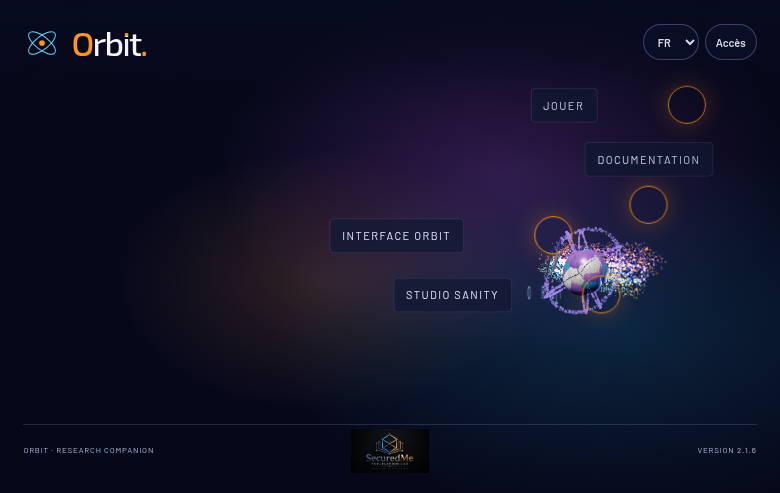
\includegraphics[width=0.85\linewidth,height=\textheight,keepaspectratio,alt={Le maintien de quatre secondes transforme le logo décoratif en ASCII et rassemble les particules. Capture du contrôle public.}]{figures/hold-ascii.png}
\caption{Le maintien de quatre secondes transforme le logo décoratif en
ASCII et rassemble les particules. Capture du contrôle public.}
\end{figure}

\begin{figure}
\centering
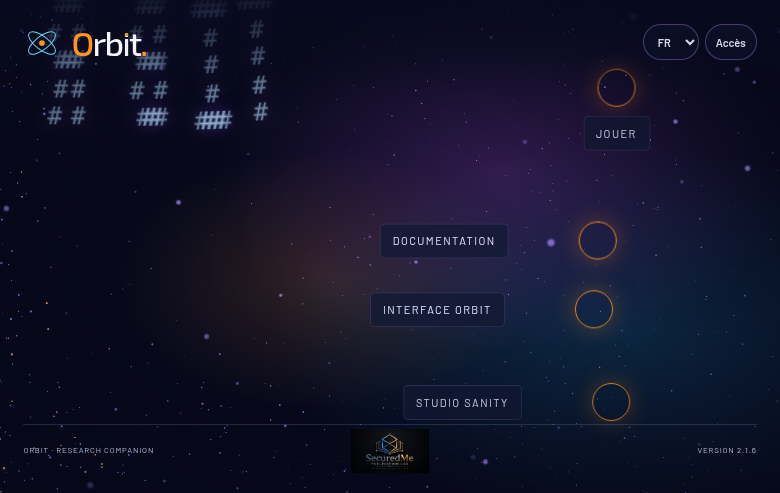
\includegraphics[width=0.85\linewidth,height=\textheight,keepaspectratio,alt={Après le collapse bref du seuil de six secondes, les particules et les lettres sont projetées vers l'extérieur. Capture du contrôle public.}]{figures/hold-explosion.png}
\caption{Après le collapse bref du seuil de six secondes, les particules
et les lettres sont projetées vers l'extérieur. Capture du contrôle
public.}
\end{figure}

Dans le catalogue, chaque mode examine une seule idée. Choisir un jeu
nettoie son stock de travail, sauf Empreinte qui garde la composition
visible pour la capturer. Les modes restent disponibles même si leurs
mécanismes coexistent déjà sur le landing. Les liens de navigation se
trouvent hors du canvas : le geste de retour ne les remplace pas.

\subsection{5. Fronde --- Position, vitesse et
amortissement}\label{fronde-position-vitesse-et-amortissement}

\textbf{Geste.} Maintenez dans la scène, tirez la perle ambre, puis
relâchez. La perle part vers le noyau et repousse visuellement les
poussières.

\begin{figure}
\centering
\pandocbounded{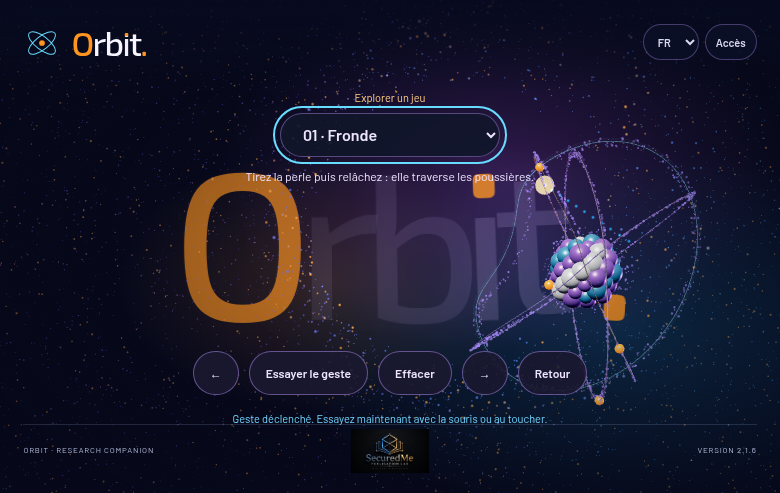
\includegraphics[keepaspectratio,alt={Fronde : état obtenu par la démonstration sur le domaine public, navigateur E2B piloté depuis Kaggle.}]{figures/sling.png}}
\caption{Fronde : état obtenu par la démonstration sur le domaine
public, navigateur E2B piloté depuis Kaggle.}
\end{figure}

\subsubsection{Comprendre avant de
calculer}\label{comprendre-avant-de-calculer}

Une position indique où se trouve la perle. Une vitesse indique comment
cette position change. Le ressort imaginaire est le segment qui relie la
perle au noyau : plus vous l'étirez, plus l'impulsion est grande,
jusqu'au plafond prévu. Le ruban lumineux rend le trajet visible ; il ne
calcule pas la trajectoire.

\subsubsection{Le mécanisme et un
exemple}\label{le-muxe9canisme-et-un-exemple}

À la libération, v = 3(a − p), bornée à 8 unités de scène par seconde. a
est la position du noyau, p celle de la perle. Ensuite p devient p + vΔt
et v devient v exp(−0,55Δt). Δt est le temps écoulé, en secondes. Pour
a=(0,0), p=(1,0), l'impulsion vaut (−3,0). Pendant 0,1 seconde, le
déplacement initial est −0,3 unité ; l'amortissement réduit ensuite la
vitesse à environ −2,84. Aux bords, la composante de vitesse est
multipliée par −0,8.

\subsubsection{Retrouver le code}\label{retrouver-le-code}

Extrait réel : \texttt{web/src/lib/atom-playground.ts}, ligne 191 dans
l'instantané de cette édition. Les retours à la ligne ont été ajoutés
après les points-virgules pour la lecture ; les instructions sont
conservées. Retrouvez aussi le marqueur
\texttt{slingVelocity.copy(atomPosition)} si les lignes ont changé.

\begin{Shaded}
\begin{Highlighting}[]
\KeywordTok{const}\NormalTok{ release}\OperatorTok{=}\NormalTok{(e}\OperatorTok{:}\BuiltInTok{PointerEvent}\NormalTok{)}\KeywordTok{=\textgreater{}}\NormalTok{\{}\ControlFlowTok{if}\NormalTok{(}\OperatorTok{!}\NormalTok{active)\{ambientHolding}\OperatorTok{=}\KeywordTok{false}\OperatorTok{;}
\NormalTok{vacuum}\OperatorTok{=}\DecValTok{0}\OperatorTok{;}
\ControlFlowTok{if}\NormalTok{(c}\OperatorTok{.}\AttributeTok{canvas}\OperatorTok{.}\FunctionTok{hasPointerCapture}\NormalTok{(e}\OperatorTok{.}\AttributeTok{pointerId}\NormalTok{))c}\OperatorTok{.}\AttributeTok{canvas}\OperatorTok{.}\FunctionTok{releasePointerCapture}\NormalTok{(e}\OperatorTok{.}\AttributeTok{pointerId}\NormalTok{)}\OperatorTok{;}
\ControlFlowTok{if}\NormalTok{(held)\{}\FunctionTok{finishRewind}\NormalTok{()}\OperatorTok{;}
\ControlFlowTok{if}\NormalTok{(c}\OperatorTok{.}\AttributeTok{canvas}\OperatorTok{.}\FunctionTok{hasPointerCapture}\NormalTok{(e}\OperatorTok{.}\AttributeTok{pointerId}\NormalTok{))c}\OperatorTok{.}\AttributeTok{canvas}\OperatorTok{.}\FunctionTok{releasePointerCapture}\NormalTok{(e}\OperatorTok{.}\AttributeTok{pointerId}\NormalTok{)}\OperatorTok{;}
\FunctionTok{message}\NormalTok{(}\StringTok{\textquotesingle{}Parcours repris · un nouveau mouvement crée une nouvelle suite.\textquotesingle{}}\NormalTok{)}\OperatorTok{;}
\NormalTok{c}\OperatorTok{.}\FunctionTok{schedule}\NormalTok{()}\OperatorTok{;}
\NormalTok{\}}\ControlFlowTok{return}\OperatorTok{;}
\NormalTok{\}}
\ControlFlowTok{if}\NormalTok{(held}\OperatorTok{\&\&}\NormalTok{mode}\OperatorTok{===}\StringTok{\textquotesingle{}sling\textquotesingle{}}\NormalTok{)\{slingVelocity}\OperatorTok{.}\FunctionTok{copy}\NormalTok{(atomPosition)}\OperatorTok{.}\FunctionTok{sub}\NormalTok{(slingPosition)}\OperatorTok{.}\FunctionTok{multiplyScalar}\NormalTok{(}\DecValTok{3}\NormalTok{)}\OperatorTok{.}\FunctionTok{clampLength}\NormalTok{(}\DecValTok{0}\OperatorTok{,}\DecValTok{8}\NormalTok{)}\OperatorTok{;}
\FunctionTok{message}\NormalTok{(}\StringTok{\textquotesingle{}Fronde relâchée : direction vers le noyau.\textquotesingle{}}\NormalTok{)}\OperatorTok{;}
\NormalTok{\}}
\end{Highlighting}
\end{Shaded}

\subsubsection{Vérifier et comprendre la
portée}\label{vuxe9rifier-et-comprendre-la-portuxe9e}

La perle rebondit sur les bords du champ de caméra. Les poussières sont
déformées par un shader : elles ne reçoivent pas une collision particule
par particule. Cette fronde est une illustration, pas un simulateur
balistique calibré.

La validation cloud a contrôlé un signal de l'effet et l'absence de
valeur non finie après un geste natif. La capture ci-dessus montre un
état rendu. Cette combinaison protège un parcours précis ; votre essai
manuel vérifie aussi la sensation et la compréhension du geste. Le
bouton de démonstration constitue une aide, distincte d'une réalisation
autonome.

\subsubsection{Exercice à faire dans une copie de
développement}\label{exercice-uxe0-faire-dans-une-copie-de-duxe9veloppement}

Remplacez le multiplicateur 3 par 2 dans une copie de développement.
Prédisez l'effet pour le même étirement, puis comparez. Conservez le
plafond de 8. Avant d'exécuter, écrivez votre prédiction. Après l'essai,
relevez ce que vous avez observé et une limite. Les pistes de correction
sont regroupées à la fin du manuel.

\subsection{6. Pinceau --- Buffer circulaire et durée de
vie}\label{pinceau-buffer-circulaire-et-duruxe9e-de-vie}

\textbf{Geste.} Déplacez le noyau dans la scène : le trajet produit un
ruban cyan. Utilisez le geste habituel de déplacement de l'atome, puis
observez le ruban s'effacer.

\begin{figure}
\centering
\pandocbounded{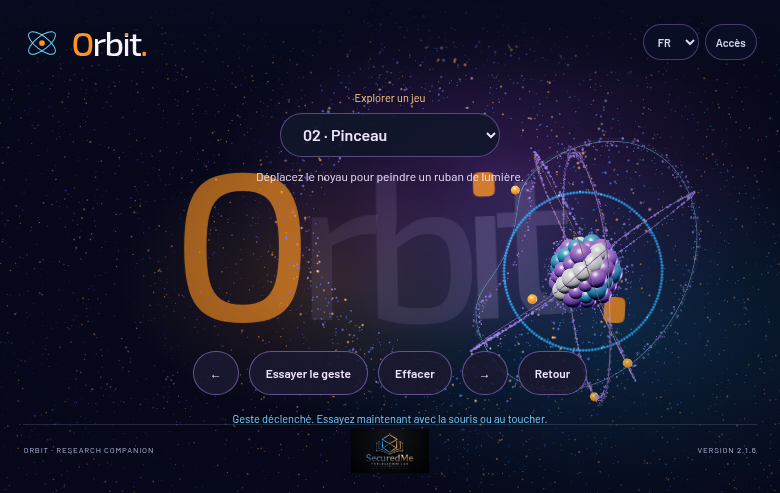
\includegraphics[keepaspectratio,alt={Pinceau : état obtenu par la démonstration sur le domaine public, navigateur E2B piloté depuis Kaggle.}]{figures/paint.png}}
\caption{Pinceau : état obtenu par la démonstration sur le domaine
public, navigateur E2B piloté depuis Kaggle.}
\end{figure}

\subsubsection{Comprendre avant de
calculer}\label{comprendre-avant-de-calculer-1}

Le pinceau garde des positions déjà traversées. Chaque point dispose
d'une réserve de visibilité appelée durée de vie. Le mouvement en crée
de nouveaux, tandis que les anciens perdent progressivement leur
opacité. Un stock fixe évite que le dessin consomme toujours plus de
mémoire.

\subsubsection{Le mécanisme et un
exemple}\label{le-muxe9canisme-et-un-exemple-1}

Le tableau contient 1 024 emplacements. emit écrit dans trailIndex, puis
avance avec (trailIndex + 1) modulo 1 024. Chaque vie α diminue de
0,22Δt jusqu'à zéro. Un point de vie initiale 1 peut donc rester actif
environ 4,55 secondes à cadence temporelle normale. Trois points sont
émis par frame lorsque le pointeur est tenu ou que la vitesse du noyau
dépasse 0,1. Le nombre émis par seconde dépend donc encore de la
fréquence de rendu.

\subsubsection{Retrouver le code}\label{retrouver-le-code-1}

Extrait réel : \texttt{web/src/lib/atom-playground.ts}, ligne 93 dans
l'instantané de cette édition. Les retours à la ligne ont été ajoutés
après les points-virgules pour la lecture ; les instructions sont
conservées. Retrouvez aussi le marqueur \texttt{function\ emit(p:} si
les lignes ont changé.

\begin{Shaded}
\begin{Highlighting}[]
\KeywordTok{function} \FunctionTok{emit}\NormalTok{(p}\OperatorTok{:}\NormalTok{THREE}\OperatorTok{.}\AttributeTok{Vector3}\OperatorTok{,}\NormalTok{life}\OperatorTok{=}\DecValTok{1}\NormalTok{)\{p}\OperatorTok{.}\FunctionTok{toArray}\NormalTok{(trailArray}\OperatorTok{,}\NormalTok{trailIndex}\OperatorTok{*}\DecValTok{3}\NormalTok{)}\OperatorTok{;}
\NormalTok{trailAlpha[trailIndex]}\OperatorTok{=}\NormalTok{life}\OperatorTok{;}
\NormalTok{trailIndex}\OperatorTok{=}\NormalTok{(trailIndex}\OperatorTok{+}\DecValTok{1}\NormalTok{)}\OperatorTok{\%}\NormalTok{trailSize}\OperatorTok{;}
\NormalTok{\}}
\end{Highlighting}
\end{Shaded}

\subsubsection{Vérifier et comprendre la
portée}\label{vuxe9rifier-et-comprendre-la-portuxe9e-1}

Le bouton Essayer trace un cercle de démonstration. Il ne remplace pas
votre parcours. Ce pinceau ne conserve pas le dessin après rechargement.
L'émission par frame peut donner une densité différente selon la
machine.

La validation cloud a contrôlé un signal de l'effet et l'absence de
valeur non finie après un geste natif. La capture ci-dessus montre un
état rendu. Cette combinaison protège un parcours précis ; votre essai
manuel vérifie aussi la sensation et la compréhension du geste. Le
bouton de démonstration constitue une aide, distincte d'une réalisation
autonome.

\subsubsection{Exercice à faire dans une copie de
développement}\label{exercice-uxe0-faire-dans-une-copie-de-duxe9veloppement-1}

Changez le coefficient d'extinction de 0,22 à 0,44. Préparez deux
captures à temps comparable et décrivez ce qui change. La capacité du
stock reste 1 024. Avant d'exécuter, écrivez votre prédiction. Après
l'essai, relevez ce que vous avez observé et une limite. Les pistes de
correction sont regroupées à la fin du manuel.

\subsection{7. Cordes --- Onde et
amplitude}\label{cordes-onde-et-amplitude}

\textbf{Geste.} Maintenez puis tirez dans la scène pour exciter les
orbites. Relâchez et observez les vibrations diminuer.

\begin{figure}
\centering
\pandocbounded{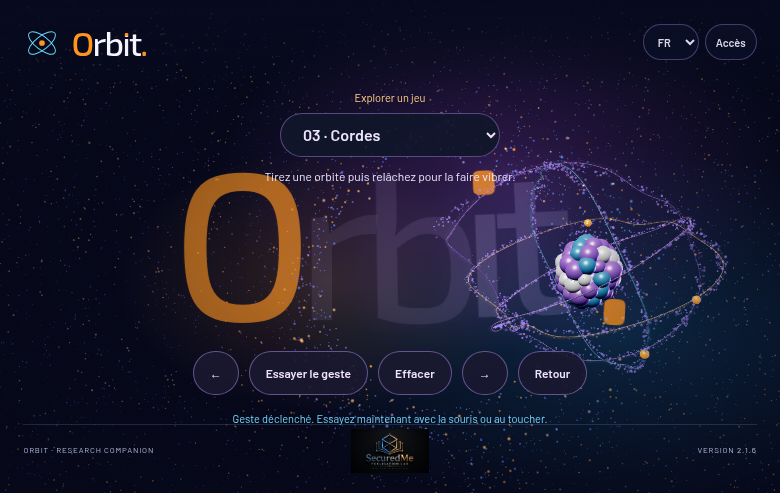
\includegraphics[keepaspectratio,alt={Cordes : état obtenu par la démonstration sur le domaine public, navigateur E2B piloté depuis Kaggle.}]{figures/strings.png}}
\caption{Cordes : état obtenu par la démonstration sur le domaine
public, navigateur E2B piloté depuis Kaggle.}
\end{figure}

\subsubsection{Comprendre avant de
calculer}\label{comprendre-avant-de-calculer-2}

Une corde peut onduler alors que son tracé moyen reste en place. Ici,
l'orbite reçoit un décalage périodique. L'étirement du geste augmente
l'amplitude ; le temps déplace les crêtes. Séparer ces deux effets évite
de confondre intensité et fréquence.

\subsubsection{Le mécanisme et un
exemple}\label{le-muxe9canisme-et-un-exemple-2}

Le décalage vaut 0,12r sin(5θ − 8t) exp(−0,1\textbar z\textbar). θ est
l'angle d'un point de l'orbite, t le temps de scène et r la force du
geste, bornée à 1,5. Le facteur 5 règle le nombre de variations
angulaires ; 8 règle la progression temporelle. Après libération, r est
multiplié par exp(−1,4Δt). Après une seconde, il reste environ 25 \% de
l'amplitude initiale.

\subsubsection{Retrouver le code}\label{retrouver-le-code-2}

Extrait réel : \texttt{web/src/lib/atom-playground.ts}, ligne 254 dans
l'instantané de cette édition. Les retours à la ligne ont été ajoutés
après les points-virgules pour la lecture ; les instructions sont
conservées. Retrouvez aussi le marqueur \texttt{ringOffset:} si les
lignes ont changé.

\begin{Shaded}
\begin{Highlighting}[]
\NormalTok{ringOffset}\OperatorTok{:}\NormalTok{(x}\OperatorTok{:}\DataTypeTok{number}\OperatorTok{,}\NormalTok{y}\OperatorTok{:}\DataTypeTok{number}\OperatorTok{,}\NormalTok{z}\OperatorTok{:}\DataTypeTok{number}\NormalTok{)}\KeywordTok{=\textgreater{}}\NormalTok{active}\OperatorTok{\&\&}\NormalTok{mode}\OperatorTok{===}\StringTok{\textquotesingle{}strings\textquotesingle{}}\OperatorTok{?}\BuiltInTok{Math}\OperatorTok{.}\FunctionTok{sin}\NormalTok{(}\BuiltInTok{Math}\OperatorTok{.}\FunctionTok{atan2}\NormalTok{(y}\OperatorTok{,}\NormalTok{x)}\OperatorTok{*}\DecValTok{5}\OperatorTok{{-}}\NormalTok{age}\OperatorTok{*}\DecValTok{8}\NormalTok{)}\OperatorTok{*}\NormalTok{ripple}\OperatorTok{*}\BuiltInTok{Math}\OperatorTok{.}\FunctionTok{exp}\NormalTok{(}\OperatorTok{{-}}\BuiltInTok{Math}\OperatorTok{.}\FunctionTok{abs}\NormalTok{(z)}\OperatorTok{*.}\DecValTok{1}\NormalTok{)}\OperatorTok{*.}\DecValTok{12}\OperatorTok{:}\DecValTok{0}\OperatorTok{,}
\end{Highlighting}
\end{Shaded}

\subsubsection{Vérifier et comprendre la
portée}\label{vuxe9rifier-et-comprendre-la-portuxe9e-2}

Le geste excite l'ensemble des orbites ; il ne sélectionne pas une corde
précise par collision. Les lignes ne sont pas un réseau de masses
reliées par des ressorts. L'onde est ajoutée au tracé existant.

La validation cloud a contrôlé un signal de l'effet et l'absence de
valeur non finie après un geste natif. La capture ci-dessus montre un
état rendu. Cette combinaison protège un parcours précis ; votre essai
manuel vérifie aussi la sensation et la compréhension du geste. Le
bouton de démonstration constitue une aide, distincte d'une réalisation
autonome.

\subsubsection{Exercice à faire dans une copie de
développement}\label{exercice-uxe0-faire-dans-une-copie-de-duxe9veloppement-2}

Comparez le facteur angulaire 5 avec 3 en gardant 8 et 0,12. Dessinez
les crêtes attendues avant la modification. Avant d'exécuter, écrivez
votre prédiction. Après l'essai, relevez ce que vous avez observé et une
limite. Les pistes de correction sont regroupées à la fin du manuel.

\subsection{8. Élastique --- Ressort amorti et déformation
localisée}\label{uxe9lastique-ressort-amorti-et-duxe9formation-localisuxe9e}

\textbf{Geste.} Pressez puis tirez dans la scène. Le noyau se déforme
localement ; relâchez pour voir son retour.

\begin{figure}
\centering
\pandocbounded{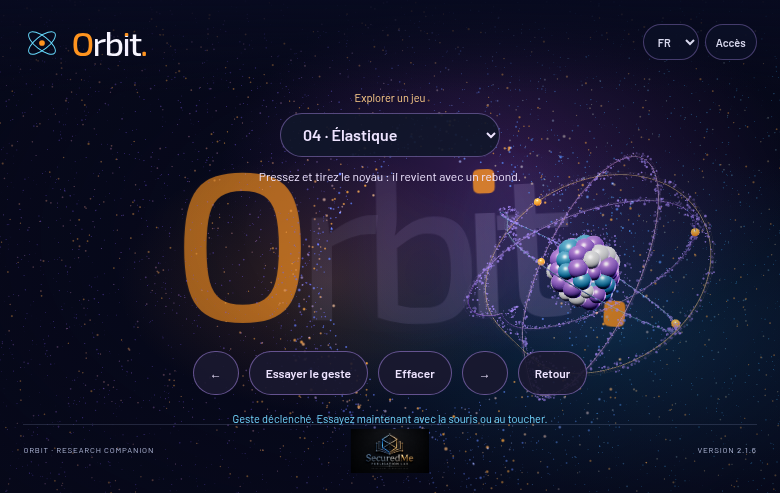
\includegraphics[keepaspectratio,alt={Élastique : état obtenu par la démonstration sur le domaine public, navigateur E2B piloté depuis Kaggle.}]{figures/elastic.png}}
\caption{Élastique : état obtenu par la démonstration sur le domaine
public, navigateur E2B piloté depuis Kaggle.}
\end{figure}

\subsubsection{Comprendre avant de
calculer}\label{comprendre-avant-de-calculer-3}

La déformation possède une position et une vitesse de retour. Une force
attire cette position vers le repos, tandis qu'un amortissement calme
les rebonds. Les pièces proches de la direction du geste bougent
davantage que les pièces éloignées.

\subsubsection{Le mécanisme et un
exemple}\label{le-muxe9canisme-et-un-exemple-3}

Avec s la déformation et w sa vitesse, le code avance w de (−18s −
4w)Δt, puis s de wΔt. Le geste borne s à 0,8. Chaque pièce reçoit
ensuite une fraction de s pondérée par exp(−4d²), où d mesure sa
distance à une zone de référence. Si s=0,5 et w=0, avec Δt=0,016, la
première variation de vitesse vaut −0,144 ; le déplacement s diminue
ensuite d'environ 0,0023.

\subsubsection{Retrouver le code}\label{retrouver-le-code-3}

Extrait réel : \texttt{web/src/lib/atom-playground.ts}, ligne 221 dans
l'instantané de cette édition. Les retours à la ligne ont été ajoutés
après les points-virgules pour la lecture ; les instructions sont
conservées. Retrouvez aussi le marqueur \texttt{springV+=} si les lignes
ont changé.

\begin{Shaded}
\begin{Highlighting}[]
\ControlFlowTok{if}\NormalTok{(mode}\OperatorTok{===}\StringTok{\textquotesingle{}elastic\textquotesingle{}}\OperatorTok{\&\&!}\NormalTok{held}\OperatorTok{\&\&}\NormalTok{moving)\{springV}\OperatorTok{+=}\NormalTok{(}\OperatorTok{{-}}\DecValTok{18}\OperatorTok{*}\NormalTok{spring}\OperatorTok{{-}}\DecValTok{4}\OperatorTok{*}\NormalTok{springV)}\OperatorTok{*}\NormalTok{dt}\OperatorTok{;}
\NormalTok{spring}\OperatorTok{+=}\NormalTok{springV}\OperatorTok{*}\NormalTok{dt}\OperatorTok{;}
\NormalTok{\}}
\end{Highlighting}
\end{Shaded}

\subsubsection{Vérifier et comprendre la
portée}\label{vuxe9rifier-et-comprendre-la-portuxe9e-3}

Les pièces du noyau se déplacent ; aucun corps mou continu n'est
calculé. Les coefficients expriment une réponse visuelle, pas une
rigidité mesurée d'un matériau. Le mouvement réduit limite l'évolution
automatique.

La validation cloud a contrôlé un signal de l'effet et l'absence de
valeur non finie après un geste natif. La capture ci-dessus montre un
état rendu. Cette combinaison protège un parcours précis ; votre essai
manuel vérifie aussi la sensation et la compréhension du geste. Le
bouton de démonstration constitue une aide, distincte d'une réalisation
autonome.

\subsubsection{Exercice à faire dans une copie de
développement}\label{exercice-uxe0-faire-dans-une-copie-de-duxe9veloppement-3}

Passez l'amortissement de 4 à 6 en conservant 18. Comparez les rebonds.
Revenez à 4 avant une autre expérience. Avant d'exécuter, écrivez votre
prédiction. Après l'essai, relevez ce que vous avez observé et une
limite. Les pistes de correction sont regroupées à la fin du manuel.

\subsection{9. Vortex --- Champ spatial et
interpolation}\label{vortex-champ-spatial-et-interpolation}

\textbf{Geste.} C'est le jeu sélectionné à l'ouverture. Maintenez puis
dessinez un cercle pour déplacer le centre du tourbillon ; relâchez pour
le laisser décroître.

\begin{figure}
\centering
\pandocbounded{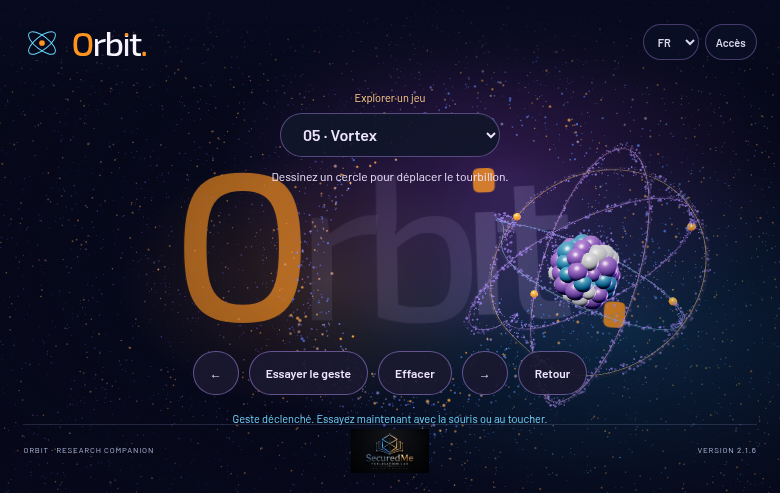
\includegraphics[keepaspectratio,alt={Vortex : état obtenu par la démonstration sur le domaine public, navigateur E2B piloté depuis Kaggle.}]{figures/vortex.png}}
\caption{Vortex : état obtenu par la démonstration sur le domaine
public, navigateur E2B piloté depuis Kaggle.}
\end{figure}

\subsubsection{Comprendre avant de
calculer}\label{comprendre-avant-de-calculer-4}

Un champ décrit une action différente selon l'endroit. Les poussières
proches du centre sont davantage tournées que les poussières éloignées.
Le centre suit votre geste avec un léger retard pour que son déplacement
reste doux.

\subsubsection{Le mécanisme et un
exemple}\label{le-muxe9canisme-et-un-exemple-4}

vortex.lerp(pointer,0.15) rapproche le centre de 15 \% de l'écart à
chaque événement de déplacement. Pour un centre à 0 et une cible à 2, le
premier pas donne 0,3. Dans le shader, l'influence vaut exp(−d²/5)
multipliée par strength. Un angle sin(0,8t) × influence × 2,4 tourne les
positions autour du centre. Après libération, strength est amortie par
exp(−0,07Δt). Cette décroissance est lente : après dix secondes, il
reste environ la moitié.

\subsubsection{Retrouver le code}\label{retrouver-le-code-4}

Extrait réel : \texttt{web/src/lib/atom-playground.ts}, ligne 183 dans
l'instantané de cette édition. Les retours à la ligne ont été ajoutés
après les points-virgules pour la lecture ; les instructions sont
conservées. Retrouvez aussi le marqueur \texttt{vortex.lerp(pointer} si
les lignes ont changé.

\begin{Shaded}
\begin{Highlighting}[]
\NormalTok{c}\OperatorTok{.}\AttributeTok{canvas}\OperatorTok{.}\FunctionTok{addEventListener}\NormalTok{(}\StringTok{\textquotesingle{}pointermove\textquotesingle{}}\OperatorTok{,}\NormalTok{e}\KeywordTok{=\textgreater{}}\NormalTok{\{}\FunctionTok{point}\NormalTok{(e)}\OperatorTok{;}
\ControlFlowTok{if}\NormalTok{(}\OperatorTok{!}\NormalTok{active)\{}\ControlFlowTok{if}\NormalTok{(starStarted}\OperatorTok{\textless{}}\DecValTok{0}\NormalTok{)vortex}\OperatorTok{.}\FunctionTok{lerp}\NormalTok{(pointer}\OperatorTok{,.}\DecValTok{15}\NormalTok{)}\OperatorTok{;}
\NormalTok{strength}\OperatorTok{=}\DecValTok{1}\OperatorTok{;}
\ControlFlowTok{if}\NormalTok{(held)e}\OperatorTok{.}\FunctionTok{stopImmediatePropagation}\NormalTok{()}\OperatorTok{;}
\NormalTok{c}\OperatorTok{.}\FunctionTok{schedule}\NormalTok{()}\OperatorTok{;}
\ControlFlowTok{return}\OperatorTok{;}
\NormalTok{\}}
\ControlFlowTok{if}\NormalTok{(held)\{}
\end{Highlighting}
\end{Shaded}

\subsubsection{Vérifier et comprendre la
portée}\label{vuxe9rifier-et-comprendre-la-portuxe9e-4}

Les positions de base des poussières restent dans leur buffer ; le
shader produit leur déplacement visuel. La rotation est périodique et
peut changer de sens. Il ne s'agit pas d'une simulation de fluide. Le
lissage dépend du nombre d'événements du pointeur.

La validation cloud a contrôlé un signal de l'effet et l'absence de
valeur non finie après un geste natif. La capture ci-dessus montre un
état rendu. Cette combinaison protège un parcours précis ; votre essai
manuel vérifie aussi la sensation et la compréhension du geste. Le
bouton de démonstration constitue une aide, distincte d'une réalisation
autonome.

\subsubsection{Exercice à faire dans une copie de
développement}\label{exercice-uxe0-faire-dans-une-copie-de-duxe9veloppement-4}

Comparez une interpolation 0,15 avec 0,4 pour un même mouvement.
Distinguez la réaction du centre et la décroissance de force. Avant
d'exécuter, écrivez votre prédiction. Après l'essai, relevez ce que vous
avez observé et une limite. Les pistes de correction sont regroupées à
la fin du manuel.

\subsection{10. Sculpter Orbit --- Échantillonnage et positions de
repos}\label{sculpter-orbit-uxe9chantillonnage-et-positions-de-repos}

\textbf{Geste.} Déplacez l'atome à travers les lettres du fond. En mode
Sculpter Orbit, ces lettres sont de vrais points Three.js qui se
déforment puis retrouvent leur tracé.

\begin{figure}
\centering
\pandocbounded{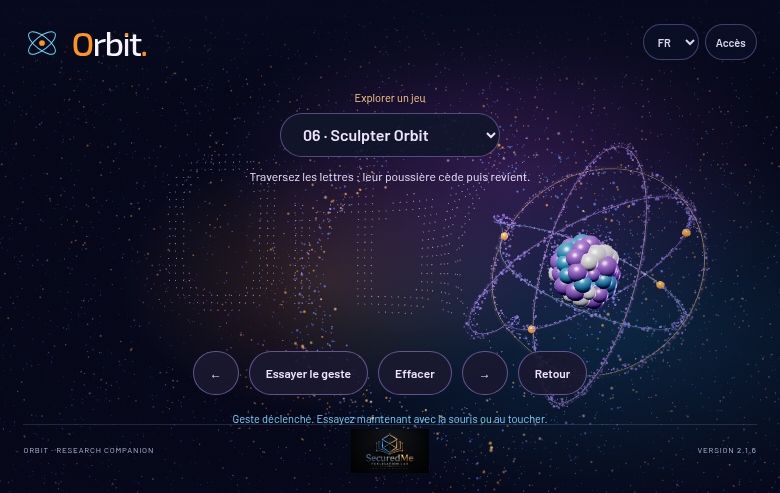
\includegraphics[keepaspectratio,alt={Sculpter Orbit : état obtenu par la démonstration sur le domaine public, navigateur E2B piloté depuis Kaggle.}]{figures/logo.png}}
\caption{Sculpter Orbit : état obtenu par la démonstration sur le
domaine public, navigateur E2B piloté depuis Kaggle.}
\end{figure}

\subsubsection{Comprendre avant de
calculer}\label{comprendre-avant-de-calculer-5}

Pour créer des lettres en particules, le programme commence par dessiner
leurs caractères sur un canvas invisible. Il lit ensuite quelques pixels
opaques et place un point à chacun de ces endroits. Chaque point possède
une adresse de repos : la forme peut céder tout en restant
reconnaissable.

\subsubsection{Le mécanisme et un
exemple}\label{le-muxe9canisme-et-un-exemple-5}

Le code échantillonne tous les sept pixels et garde les pixels dont
l'alpha dépasse 80. Les positions sont converties du rectangle de
l'écran vers le plan de scène. La force locale comporte exp(−d²/1,2) ×
0,9 ; une impulsion de démonstration ajoute 0,6 exp(−1,8t). Le point est
repoussé dans la direction qui l'éloigne du noyau. Une fois le noyau
loin, sa position calculée redevient proche de sa position de repos.

\subsubsection{Retrouver le code}\label{retrouver-le-code-5}

Extrait réel : \texttt{web/src/lib/atom-playground.ts}, ligne 232 dans
l'instantané de cette édition. Les retours à la ligne ont été ajoutés
après les points-virgules pour la lecture ; les instructions sont
conservées. Retrouvez aussi le marqueur \texttt{logoPositions{[}i{]}=}
si les lignes ont changé.

\begin{Shaded}
\begin{Highlighting}[]
\ControlFlowTok{if}\NormalTok{(mode}\OperatorTok{===}\StringTok{\textquotesingle{}logo\textquotesingle{}}\NormalTok{)\{}\FunctionTok{buildLogo}\NormalTok{()}\OperatorTok{;}
\ControlFlowTok{if}\NormalTok{(logoAge}\OperatorTok{\textgreater{}=}\DecValTok{0}\NormalTok{)logoAge}\OperatorTok{+=}\NormalTok{dt}\OperatorTok{;}
\ControlFlowTok{for}\NormalTok{(}\KeywordTok{let}\NormalTok{ i}\OperatorTok{=}\DecValTok{0}\OperatorTok{;}
\NormalTok{i}\OperatorTok{\textless{}}\NormalTok{logoPositions}\OperatorTok{.}\AttributeTok{length}\OperatorTok{;}
\NormalTok{i}\OperatorTok{+=}\DecValTok{3}\NormalTok{)\{}\KeywordTok{const}\NormalTok{ dx}\OperatorTok{=}\NormalTok{logoHomes[i]}\OperatorTok{{-}}\NormalTok{atomPosition}\OperatorTok{.}\AttributeTok{x}\OperatorTok{,}\NormalTok{dy}\OperatorTok{=}\NormalTok{logoHomes[i}\OperatorTok{+}\DecValTok{1}\NormalTok{]}\OperatorTok{{-}}\NormalTok{atomPosition}\OperatorTok{.}\AttributeTok{y}\OperatorTok{,}\NormalTok{d}\OperatorTok{=}\BuiltInTok{Math}\OperatorTok{.}\FunctionTok{hypot}\NormalTok{(dx}\OperatorTok{,}\NormalTok{dy)}\OperatorTok{||}\DecValTok{1}\OperatorTok{;}
\KeywordTok{const}\NormalTok{ force}\OperatorTok{=}\BuiltInTok{Math}\OperatorTok{.}\FunctionTok{exp}\NormalTok{(}\OperatorTok{{-}}\NormalTok{d}\OperatorTok{*}\NormalTok{d}\OperatorTok{/}\FloatTok{1.2}\NormalTok{)}\OperatorTok{*.}\DecValTok{9}\OperatorTok{+}\NormalTok{(logoAge}\OperatorTok{\textgreater{}=}\DecValTok{0}\OperatorTok{?}\BuiltInTok{Math}\OperatorTok{.}\FunctionTok{exp}\NormalTok{(}\OperatorTok{{-}}\NormalTok{logoAge}\OperatorTok{*}\FloatTok{1.8}\NormalTok{)}\OperatorTok{*.}\DecValTok{6}\OperatorTok{:}\DecValTok{0}\NormalTok{)}\OperatorTok{;}
\NormalTok{logoPositions[i]}\OperatorTok{=}\NormalTok{logoHomes[i]}\OperatorTok{+}\NormalTok{dx}\OperatorTok{/}\NormalTok{d}\OperatorTok{*}\NormalTok{force}\OperatorTok{;}
\NormalTok{logoPositions[i}\OperatorTok{+}\DecValTok{1}\NormalTok{]}\OperatorTok{=}\NormalTok{logoHomes[i}\OperatorTok{+}\DecValTok{1}\NormalTok{]}\OperatorTok{+}\NormalTok{dy}\OperatorTok{/}\NormalTok{d}\OperatorTok{*}\NormalTok{force}\OperatorTok{;}
\NormalTok{logoPositions[i}\OperatorTok{+}\DecValTok{2}\NormalTok{]}\OperatorTok{=}\BuiltInTok{Math}\OperatorTok{.}\FunctionTok{sin}\NormalTok{(i}\OperatorTok{+}\NormalTok{age)}\OperatorTok{*}\NormalTok{force}\OperatorTok{*.}\DecValTok{15}\OperatorTok{;}
\NormalTok{\}logoGeometry}\OperatorTok{.}\AttributeTok{attributes}\OperatorTok{.}\AttributeTok{position}\OperatorTok{.}\AttributeTok{needsUpdate}\OperatorTok{=}\KeywordTok{true}\OperatorTok{;}
\NormalTok{\}}
\end{Highlighting}
\end{Shaded}

\subsubsection{Vérifier et comprendre la
portée}\label{vuxe9rifier-et-comprendre-la-portuxe9e-5}

La reconstruction est recalculée quand les dimensions changent. La
lisibilité dépend de la police chargée et de la taille de l'écran. Le
retour est calculé à partir de la distance et de l'impulsion ; ce n'est
pas un ressort individuel pour chaque lettre.

La validation cloud a contrôlé un signal de l'effet et l'absence de
valeur non finie après un geste natif. La capture ci-dessus montre un
état rendu. Cette combinaison protège un parcours précis ; votre essai
manuel vérifie aussi la sensation et la compréhension du geste. Le
bouton de démonstration constitue une aide, distincte d'une réalisation
autonome.

\subsubsection{Exercice à faire dans une copie de
développement}\label{exercice-uxe0-faire-dans-une-copie-de-duxe9veloppement-5}

Comparez un pas d'échantillonnage de 7 puis de 10. Observez lisibilité
et nombre de points ; restaurez 7 avant d'étudier la force. Avant
d'exécuter, écrivez votre prédiction. Après l'essai, relevez ce que vous
avez observé et une limite. Les pistes de correction sont regroupées à
la fin du manuel.

\subsection{11. Constellation --- Collection bornée et sélection de
proximité}\label{constellation-collection-bornuxe9e-et-suxe9lection-de-proximituxe9}

\textbf{Geste.} Touchez ou cliquez le fond pour ajouter une étoile.
Attrapez une étoile proche pour la déplacer. Les étoiles se relient dans
leur ordre d'ajout.

\begin{figure}
\centering
\pandocbounded{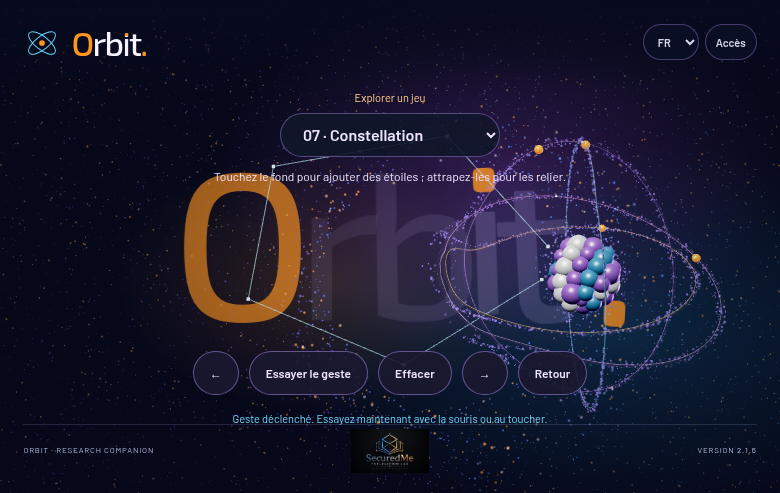
\includegraphics[keepaspectratio,alt={Constellation : état obtenu par la démonstration sur le domaine public, navigateur E2B piloté depuis Kaggle.}]{figures/stars.png}}
\caption{Constellation : état obtenu par la démonstration sur le domaine
public, navigateur E2B piloté depuis Kaggle.}
\end{figure}

\subsubsection{Comprendre avant de
calculer}\label{comprendre-avant-de-calculer-6}

Une constellation est une liste de positions. L'utilisateur crée les
éléments et le programme dessine une ligne entre eux. Pour savoir si
vous attrapez une étoile existante, le code mesure la distance entre le
pointeur et chaque position.

\subsubsection{Le mécanisme et un
exemple}\label{le-muxe9canisme-et-un-exemple-6}

Une étoile est sélectionnée si sa distance au pointeur est inférieure à
0,25 unité de scène. Si aucune n'est trouvée, une nouvelle est créée,
jusqu'à 32. Les tableaux graphiques sont préalloués. setDrawRange montre
seulement le nombre d'éléments présents. Le tracé relie la liste en
séquence : A, puis B, puis C. Ce choix exprime l'ordre de construction,
pas une relation scientifique.

\subsubsection{Retrouver le code}\label{retrouver-le-code-6}

Extrait réel : \texttt{web/src/lib/atom-playground.ts}, ligne 178 dans
l'instantané de cette édition. Les retours à la ligne ont été ajoutés
après les points-virgules pour la lecture ; les instructions sont
conservées. Retrouvez aussi le marqueur \texttt{picked=stars.findIndex}
si les lignes ont changé.

\begin{Shaded}
\begin{Highlighting}[]
\ControlFlowTok{if}\NormalTok{(mode}\OperatorTok{===}\StringTok{\textquotesingle{}stars\textquotesingle{}}\NormalTok{)\{picked}\OperatorTok{=}\NormalTok{stars}\OperatorTok{.}\FunctionTok{findIndex}\NormalTok{(p}\KeywordTok{=\textgreater{}}\NormalTok{p}\OperatorTok{.}\FunctionTok{distanceTo}\NormalTok{(pointer)}\OperatorTok{\textless{}.}\DecValTok{25}\NormalTok{)}\OperatorTok{;}
\ControlFlowTok{if}\NormalTok{(picked}\OperatorTok{\textless{}}\DecValTok{0}\OperatorTok{\&\&}\NormalTok{stars}\OperatorTok{.}\AttributeTok{length}\OperatorTok{\textless{}}\DecValTok{32}\NormalTok{)\{stars}\OperatorTok{.}\FunctionTok{push}\NormalTok{(pointer}\OperatorTok{.}\FunctionTok{clone}\NormalTok{())}\OperatorTok{;}
\NormalTok{picked}\OperatorTok{=}\NormalTok{stars}\OperatorTok{.}\AttributeTok{length}\OperatorTok{{-}}\DecValTok{1}\OperatorTok{;}
\NormalTok{\}}\FunctionTok{message}\NormalTok{(}\VerbatimStringTok{\textasciigrave{}}\SpecialCharTok{$\{}\NormalTok{stars}\OperatorTok{.}\AttributeTok{length}\SpecialCharTok{\}}\VerbatimStringTok{ étoiles dans votre constellation.\textasciigrave{}}\NormalTok{)}\OperatorTok{;}
\NormalTok{\}}
\end{Highlighting}
\end{Shaded}

\subsubsection{Vérifier et comprendre la
portée}\label{vuxe9rifier-et-comprendre-la-portuxe9e-6}

La première étoile de la liste située dans le rayon est choisie. Avec
des points rapprochés, ce n'est pas toujours la plus proche. Les liens
restent séquentiels, et la collection disparaît avec Effacer ou un
changement de jeu.

La validation cloud a contrôlé un signal de l'effet et l'absence de
valeur non finie après un geste natif. La capture ci-dessus montre un
état rendu. Cette combinaison protège un parcours précis ; votre essai
manuel vérifie aussi la sensation et la compréhension du geste. Le
bouton de démonstration constitue une aide, distincte d'une réalisation
autonome.

\subsubsection{Exercice à faire dans une copie de
développement}\label{exercice-uxe0-faire-dans-une-copie-de-duxe9veloppement-6}

Changez le rayon de sélection de 0,25 à 0,35. Prédisez l'effet lorsque
deux étoiles sont proches. Gardez la borne de 32. Avant d'exécuter,
écrivez votre prédiction. Après l'essai, relevez ce que vous avez
observé et une limite. Les pistes de correction sont regroupées à la fin
du manuel.

\subsection{12. Collection --- Accumulation, capacité et
libération}\label{collection-accumulation-capacituxe9-et-libuxe9ration}

\textbf{Geste.} Maintenez le fond pour faire grandir une couronne ambre
autour du noyau. Relâchez pour semer une trace de points.

\begin{figure}
\centering
\pandocbounded{
\includegraphics[keepaspectratio,alt={Collection : état obtenu par la démonstration sur le domaine public, navigateur E2B piloté depuis Kaggle.}]{figures/collect.png}}
\caption{Collection : état obtenu par la démonstration sur le domaine
public, navigateur E2B piloté depuis Kaggle.}
\end{figure}

\subsubsection{Comprendre avant de
calculer}\label{comprendre-avant-de-calculer-7}

Le maintien accumule une quantité. La libération change de phase : ce
qui était rangé autour du noyau devient un motif semé. Un plafond
empêche une accumulation infinie. Le vocabulaire de récolte décrit ici
une expérience visuelle.

\subsubsection{Le mécanisme et un
exemple}\label{le-muxe9canisme-et-un-exemple-7}

collecting augmente de 24Δt jusqu'à 128. Après deux secondes de
maintien, la cible nominale est 48 points. Le rayon de couronne vaut
0,85 + 0,65 × seedFlash. À la libération, les points sont placés autour
du noyau selon un pas angulaire 0,618 × 2π. Le shader rapproche aussi la
poussière du centre. La couronne et la poussière utilisent des stocks
distincts.

\subsubsection{Retrouver le code}\label{retrouver-le-code-7}

Extrait réel : \texttt{web/src/lib/atom-playground.ts}, ligne 224 dans
l'instantané de cette édition. Les retours à la ligne ont été ajoutés
après les points-virgules pour la lecture ; les instructions sont
conservées. Retrouvez aussi le marqueur
\texttt{collecting=Math.min(128,collecting+dt*24)} si les lignes ont
changé.

\begin{Shaded}
\begin{Highlighting}[]
\ControlFlowTok{if}\NormalTok{(mode}\OperatorTok{===}\StringTok{\textquotesingle{}collect\textquotesingle{}}\NormalTok{)\{}\ControlFlowTok{if}\NormalTok{(held)collecting}\OperatorTok{=}\BuiltInTok{Math}\OperatorTok{.}\FunctionTok{min}\NormalTok{(}\DecValTok{128}\OperatorTok{,}\NormalTok{collecting}\OperatorTok{+}\NormalTok{dt}\OperatorTok{*}\DecValTok{24}\NormalTok{)}\OperatorTok{;}
\NormalTok{seedFlash}\OperatorTok{=}\BuiltInTok{Math}\OperatorTok{.}\FunctionTok{max}\NormalTok{(}\DecValTok{0}\OperatorTok{,}\NormalTok{seedFlash}\OperatorTok{{-}}\NormalTok{dt}\OperatorTok{*.}\DecValTok{4}\NormalTok{)}\OperatorTok{;}
\ControlFlowTok{for}\NormalTok{(}\KeywordTok{let}\NormalTok{ i}\OperatorTok{=}\DecValTok{0}\OperatorTok{;}
\NormalTok{i}\OperatorTok{\textless{}}\DecValTok{128}\OperatorTok{;}
\NormalTok{i}\OperatorTok{++}\NormalTok{)\{}\KeywordTok{const}\NormalTok{ a}\OperatorTok{=}\NormalTok{i}\OperatorTok{/}\DecValTok{128}\OperatorTok{*}\BuiltInTok{Math}\OperatorTok{.}\ConstantTok{PI}\OperatorTok{*}\DecValTok{2}\OperatorTok{+}\NormalTok{age}\OperatorTok{*.}\DecValTok{5}\OperatorTok{,}\NormalTok{r}\OperatorTok{=.}\DecValTok{85}\OperatorTok{+}\NormalTok{seedFlash}\OperatorTok{*.}\DecValTok{65}\OperatorTok{;}
\KeywordTok{new}\NormalTok{ THREE}\OperatorTok{.}\FunctionTok{Vector3}\NormalTok{(atomPosition}\OperatorTok{.}\AttributeTok{x}\OperatorTok{+}\BuiltInTok{Math}\OperatorTok{.}\FunctionTok{cos}\NormalTok{(a)}\OperatorTok{*}\NormalTok{r}\OperatorTok{,}\NormalTok{atomPosition}\OperatorTok{.}\AttributeTok{y}\OperatorTok{+}\BuiltInTok{Math}\OperatorTok{.}\FunctionTok{sin}\NormalTok{(a)}\OperatorTok{*}\NormalTok{r}\OperatorTok{,}\BuiltInTok{Math}\OperatorTok{.}\FunctionTok{sin}\NormalTok{(a}\OperatorTok{*}\DecValTok{3}\NormalTok{)}\OperatorTok{*.}\DecValTok{15}\NormalTok{)}\OperatorTok{.}\FunctionTok{toArray}\NormalTok{(crownArray}\OperatorTok{,}\NormalTok{i}\OperatorTok{*}\DecValTok{3}\NormalTok{)}\OperatorTok{;}
\NormalTok{\}crownGeometry}\OperatorTok{.}\FunctionTok{setDrawRange}\NormalTok{(}\DecValTok{0}\OperatorTok{,}\BuiltInTok{Math}\OperatorTok{.}\FunctionTok{floor}\NormalTok{(collecting))}\OperatorTok{;}
\NormalTok{crownGeometry}\OperatorTok{.}\AttributeTok{attributes}\OperatorTok{.}\AttributeTok{position}\OperatorTok{.}\AttributeTok{needsUpdate}\OperatorTok{=}\KeywordTok{true}\OperatorTok{;}
\NormalTok{\}}
\end{Highlighting}
\end{Shaded}

\subsubsection{Vérifier et comprendre la
portée}\label{vuxe9rifier-et-comprendre-la-portuxe9e-7}

Le programme ne retire pas une particule précise du fond à chaque
récolte. Le compteur de la couronne est un état de jeu indépendant.
Parler de conservation du nombre de poussières serait inexact.

La validation cloud a contrôlé un signal de l'effet et l'absence de
valeur non finie après un geste natif. La capture ci-dessus montre un
état rendu. Cette combinaison protège un parcours précis ; votre essai
manuel vérifie aussi la sensation et la compréhension du geste. Le
bouton de démonstration constitue une aide, distincte d'une réalisation
autonome.

\subsubsection{Exercice à faire dans une copie de
développement}\label{exercice-uxe0-faire-dans-une-copie-de-duxe9veloppement-7}

Essayez une accumulation de 12Δt. Comparez le temps nécessaire pour
atteindre une quantité donnée. Conservez le maximum 128. Avant
d'exécuter, écrivez votre prédiction. Après l'essai, relevez ce que vous
avez observé et une limite. Les pistes de correction sont regroupées à
la fin du manuel.

\subsection{13. Rosaces --- Coordonnées polaires et
paramètres}\label{rosaces-coordonnuxe9es-polaires-et-paramuxe8tres}

\textbf{Geste.} Tournez le noyau : la rotation change la fleur lumineuse
tracée autour de lui.

\begin{figure}
\centering
\pandocbounded{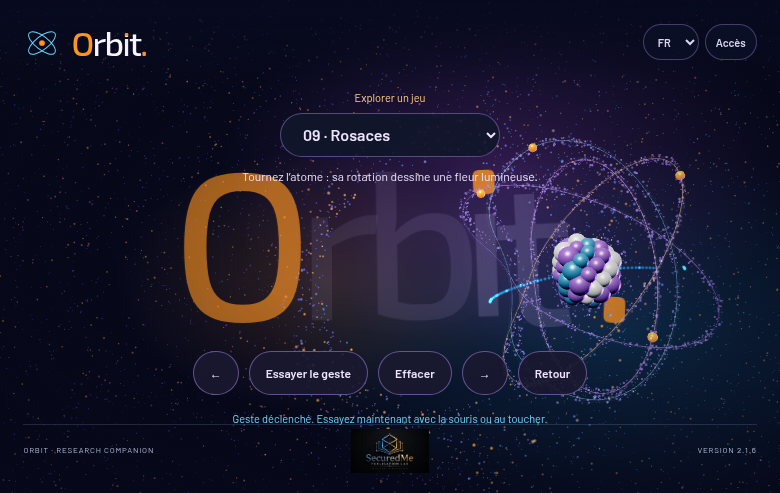
\includegraphics[keepaspectratio,alt={Rosaces : état obtenu par la démonstration sur le domaine public, navigateur E2B piloté depuis Kaggle.}]{figures/rosette.png}}
\caption{Rosaces : état obtenu par la démonstration sur le domaine
public, navigateur E2B piloté depuis Kaggle.}
\end{figure}

\subsubsection{Comprendre avant de
calculer}\label{comprendre-avant-de-calculer-8}

Un point peut être décrit par un angle et une distance au centre. Si la
distance varie régulièrement pendant que l'angle tourne, le point
dessine une fleur. Votre rotation modifie le motif ; le rendu émet les
points qui rendent ce motif visible.

\subsubsection{Le mécanisme et un
exemple}\label{le-muxe9canisme-et-un-exemple-8}

Le rayon vaut 1,25 cos(ka + y), où a est l'angle progressif, y la
rotation horizontale du noyau et k = 3 + round(2\textbar x\textbar), x
étant son autre rotation. Les coordonnées deviennent r cos(a) et r
sin(a). À a=0, y=0, r vaut 1,25 ; si ka+y vaut π/2, r est nul. Un rayon
négatif place le point de l'autre côté du centre. Les six émissions par
frame ont de petits décalages d'angle.

\subsubsection{Retrouver le code}\label{retrouver-le-code-8}

Extrait réel : \texttt{web/src/lib/atom-playground.ts}, ligne 225 dans
l'instantané de cette édition. Les retours à la ligne ont été ajoutés
après les points-virgules pour la lecture ; les instructions sont
conservées. Retrouvez aussi le marqueur \texttt{petals=3+} si les lignes
ont changé.

\begin{Shaded}
\begin{Highlighting}[]
\ControlFlowTok{if}\NormalTok{(mode}\OperatorTok{===}\StringTok{\textquotesingle{}rosette\textquotesingle{}}\NormalTok{)\{}\KeywordTok{const}\NormalTok{ rotation}\OperatorTok{=}\NormalTok{c}\OperatorTok{.}\FunctionTok{rotation}\NormalTok{()}\OperatorTok{;}
\ControlFlowTok{for}\NormalTok{(}\KeywordTok{let}\NormalTok{ i}\OperatorTok{=}\DecValTok{0}\OperatorTok{;}
\NormalTok{i}\OperatorTok{\textless{}}\DecValTok{6}\OperatorTok{;}
\NormalTok{i}\OperatorTok{++}\NormalTok{)\{}\KeywordTok{const}\NormalTok{ a}\OperatorTok{=}\NormalTok{age}\OperatorTok{*.}\DecValTok{6}\OperatorTok{+}\NormalTok{i}\OperatorTok{/}\DecValTok{6}\OperatorTok{*.}\BaseNTok{03}\OperatorTok{,}\NormalTok{petals}\OperatorTok{=}\DecValTok{3}\OperatorTok{+}\BuiltInTok{Math}\OperatorTok{.}\FunctionTok{round}\NormalTok{(}\BuiltInTok{Math}\OperatorTok{.}\FunctionTok{abs}\NormalTok{(rotation}\OperatorTok{.}\AttributeTok{x}\NormalTok{)}\OperatorTok{*}\DecValTok{2}\NormalTok{)}\OperatorTok{,}\NormalTok{r}\OperatorTok{=}\FloatTok{1.25}\OperatorTok{*}\BuiltInTok{Math}\OperatorTok{.}\FunctionTok{cos}\NormalTok{(petals}\OperatorTok{*}\NormalTok{a}\OperatorTok{+}\NormalTok{rotation}\OperatorTok{.}\AttributeTok{y}\NormalTok{)}\OperatorTok{;}
\FunctionTok{emit}\NormalTok{(atomPosition}\OperatorTok{.}\FunctionTok{clone}\NormalTok{()}\OperatorTok{.}\FunctionTok{add}\NormalTok{(}\KeywordTok{new}\NormalTok{ THREE}\OperatorTok{.}\FunctionTok{Vector3}\NormalTok{(}\BuiltInTok{Math}\OperatorTok{.}\FunctionTok{cos}\NormalTok{(a)}\OperatorTok{*}\NormalTok{r}\OperatorTok{,}\BuiltInTok{Math}\OperatorTok{.}\FunctionTok{sin}\NormalTok{(a)}\OperatorTok{*}\NormalTok{r}\OperatorTok{,.}\DecValTok{1}\NormalTok{))}\OperatorTok{,.}\DecValTok{8}\NormalTok{)}\OperatorTok{;}
\NormalTok{\}\}}
\end{Highlighting}
\end{Shaded}

\subsubsection{Vérifier et comprendre la
portée}\label{vuxe9rifier-et-comprendre-la-portuxe9e-8}

La valeur k participe au nombre de pétales, mais les roses polaires ont
des propriétés différentes pour les entiers pairs et impairs. Le nom de
variable petals n'est pas une preuve que k égale toujours le nombre
visuel de pétales. L'émission reste liée aux frames.

La validation cloud a contrôlé un signal de l'effet et l'absence de
valeur non finie après un geste natif. La capture ci-dessus montre un
état rendu. Cette combinaison protège un parcours précis ; votre essai
manuel vérifie aussi la sensation et la compréhension du geste. Le
bouton de démonstration constitue une aide, distincte d'une réalisation
autonome.

\subsubsection{Exercice à faire dans une copie de
développement}\label{exercice-uxe0-faire-dans-une-copie-de-duxe9veloppement-8}

Changez l'amplitude 1,25 à 0,9. Gardez k inchangé pour comparer la
taille seule. Avant d'exécuter, écrivez votre prédiction. Après l'essai,
relevez ce que vous avez observé et une limite. Les pistes de correction
sont regroupées à la fin du manuel.

\subsection{14. Portails --- Changement de position et
anti-rebond}\label{portails-changement-de-position-et-anti-rebond}

\textbf{Geste.} Déplacez le noyau vers le centre d'un anneau. Il ressort
par l'autre, accompagné d'un trajet lumineux.

\begin{figure}
\centering
\pandocbounded{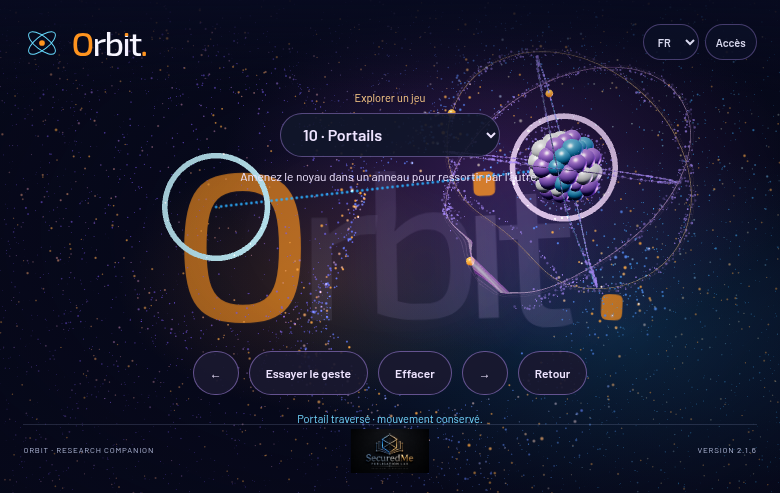
\includegraphics[keepaspectratio,alt={Portails : état obtenu par la démonstration sur le domaine public, navigateur E2B piloté depuis Kaggle.}]{figures/portals.png}}
\caption{Portails : état obtenu par la démonstration sur le domaine
public, navigateur E2B piloté depuis Kaggle.}
\end{figure}

\subsubsection{Comprendre avant de
calculer}\label{comprendre-avant-de-calculer-9}

Un portail change immédiatement la position, puis laisse le mouvement se
poursuivre. Sans délai, le noyau arrivé dans le second anneau pourrait
immédiatement revenir dans le premier. Une courte période de repos évite
cette boucle.

\subsubsection{Le mécanisme et un
exemple}\label{le-muxe9canisme-et-un-exemple-9}

L'entrée est détectée à moins de 0,5 unité du centre d'un portail. Le
déplacement ajouté vaut destination − origine. Avec les centres (−2,2 ;
0,5) et (2,2 ; 1), le transfert ajoute (4,4 ; 0,5). La vitesse existante
n'est pas réécrite. cooldown devient 1,3 seconde ; une nouvelle
traversée attend son retour à zéro. Soixante-dix points marquent le lien
entre les centres.

\subsubsection{Retrouver le code}\label{retrouver-le-code-9}

Extrait réel : \texttt{web/src/lib/atom-playground.ts}, ligne 226 dans
l'instantané de cette édition. Les retours à la ligne ont été ajoutés
après les points-virgules pour la lecture ; les instructions sont
conservées. Retrouvez aussi le marqueur
\texttt{portalCrossings++;cooldown=1.3} si les lignes ont changé.

\begin{Shaded}
\begin{Highlighting}[]
\ControlFlowTok{if}\NormalTok{(mode}\OperatorTok{===}\StringTok{\textquotesingle{}portals\textquotesingle{}}\OperatorTok{\&\&}\NormalTok{cooldown}\OperatorTok{===}\DecValTok{0}\NormalTok{)\{}\KeywordTok{const}\NormalTok{ index}\OperatorTok{=}\NormalTok{[portalA}\OperatorTok{,}\NormalTok{portalB]}\OperatorTok{.}\FunctionTok{findIndex}\NormalTok{(p}\KeywordTok{=\textgreater{}}\NormalTok{p}\OperatorTok{.}\FunctionTok{distanceTo}\NormalTok{(atomPosition)}\OperatorTok{\textless{}.}\DecValTok{5}\NormalTok{)}\OperatorTok{;}
\ControlFlowTok{if}\NormalTok{(index}\OperatorTok{\textgreater{}=}\DecValTok{0}\NormalTok{)\{}\KeywordTok{const} \ImportTok{from}\OperatorTok{=}\NormalTok{index}\OperatorTok{===}\DecValTok{0}\OperatorTok{?}\NormalTok{portalA}\OperatorTok{:}\NormalTok{portalB}\OperatorTok{,}\NormalTok{to}\OperatorTok{=}\NormalTok{index}\OperatorTok{===}\DecValTok{0}\OperatorTok{?}\NormalTok{portalB}\OperatorTok{:}\NormalTok{portalA}\OperatorTok{;}
\NormalTok{c}\OperatorTok{.}\AttributeTok{flight}\OperatorTok{.}\FunctionTok{add}\NormalTok{(}\KeywordTok{new}\NormalTok{ THREE}\OperatorTok{.}\FunctionTok{Vector2}\NormalTok{(to}\OperatorTok{.}\AttributeTok{x}\OperatorTok{{-}}\NormalTok{from}\OperatorTok{.}\AttributeTok{x}\OperatorTok{,}\NormalTok{to}\OperatorTok{.}\AttributeTok{y}\OperatorTok{{-}}\NormalTok{from}\OperatorTok{.}\AttributeTok{y}\NormalTok{))}\OperatorTok{;}
\NormalTok{portalCrossings}\OperatorTok{++;}
\NormalTok{cooldown}\OperatorTok{=}\FloatTok{1.3}\OperatorTok{;}
\ControlFlowTok{for}\NormalTok{(}\KeywordTok{let}\NormalTok{ i}\OperatorTok{=}\DecValTok{0}\OperatorTok{;}
\NormalTok{i}\OperatorTok{\textless{}}\DecValTok{70}\OperatorTok{;}
\NormalTok{i}\OperatorTok{++}\NormalTok{)}\FunctionTok{emit}\NormalTok{(from}\OperatorTok{.}\FunctionTok{clone}\NormalTok{()}\OperatorTok{.}\FunctionTok{lerp}\NormalTok{(to}\OperatorTok{,}\NormalTok{i}\OperatorTok{/}\DecValTok{69}\NormalTok{))}\OperatorTok{;}
\FunctionTok{message}\NormalTok{(}\StringTok{\textquotesingle{}Portail traversé · mouvement conservé.\textquotesingle{}}\NormalTok{)}\OperatorTok{;}
\NormalTok{\}\}}
\end{Highlighting}
\end{Shaded}

\subsubsection{Vérifier et comprendre la
portée}\label{vuxe9rifier-et-comprendre-la-portuxe9e-9}

Le seuil porte sur la distance des centres, pas sur une collision exacte
avec le tore. Aucun passage topologique ou relativiste n'est simulé. Les
positions sont fixes et la vitesse est conservée par choix d'animation.

La validation cloud a contrôlé un signal de l'effet et l'absence de
valeur non finie après un geste natif. La capture ci-dessus montre un
état rendu. Cette combinaison protège un parcours précis ; votre essai
manuel vérifie aussi la sensation et la compréhension du geste. Le
bouton de démonstration constitue une aide, distincte d'une réalisation
autonome.

\subsubsection{Exercice à faire dans une copie de
développement}\label{exercice-uxe0-faire-dans-une-copie-de-duxe9veloppement-9}

Réglez le délai à 2 secondes. Comparez la possibilité de retourner
immédiatement dans l'autre sens, puis restaurez 1,3. Avant d'exécuter,
écrivez votre prédiction. Après l'essai, relevez ce que vous avez
observé et une limite. Les pistes de correction sont regroupées à la fin
du manuel.

\subsection{15. Puzzle --- Erreur, tolérance et
succès}\label{puzzle-erreur-toluxe9rance-et-succuxe8s}

\textbf{Geste.} Tournez le noyau pour aligner ses orbites avec les
silhouettes ambre. Essayer le geste montre l'alignement assisté ;
Effacer permet une tentative manuelle.

\begin{figure}
\centering
\pandocbounded{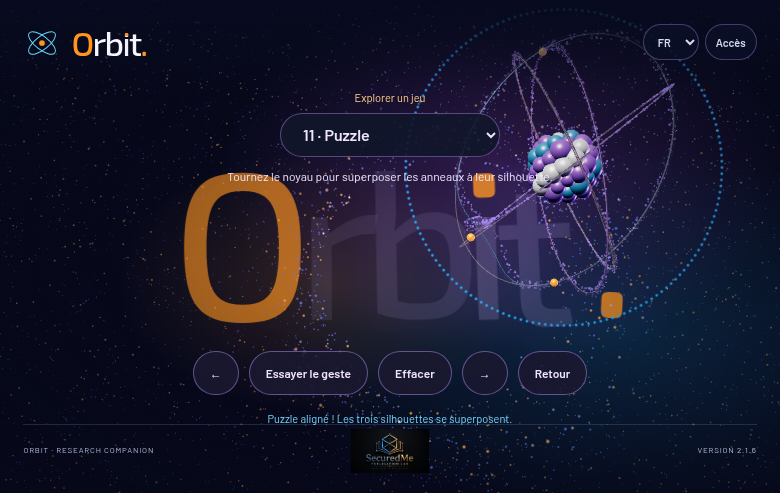
\includegraphics[keepaspectratio,alt={Puzzle : état obtenu par la démonstration sur le domaine public, navigateur E2B piloté depuis Kaggle.}]{figures/puzzle.png}}
\caption{Puzzle : état obtenu par la démonstration sur le domaine
public, navigateur E2B piloté depuis Kaggle.}
\end{figure}

\subsubsection{Comprendre avant de
calculer}\label{comprendre-avant-de-calculer-10}

Comparer exactement deux nombres flottants rendrait un jeu difficile. Le
programme mesure plutôt un écart et accepte une petite zone de réussite.
L'angle d'un cercle exige aussi de reconnaître que deux tours complets
ramènent au même endroit.

\subsubsection{Le mécanisme et un
exemple}\label{le-muxe9canisme-et-un-exemple-10}

La cible est x=0,35 radian, y=0,7 radian. L'erreur combine la différence
de x et la différence angulaire de y : hypot(Δx,
atan2(sin(Δy),cos(Δy))). Le succès est déclenché si cette norme est
inférieure à 0,12. À Δx=0,06 et Δy=0,08, la norme vaut 0,10 : la
condition est satisfaite. Un drapeau puzzleSolved évite de répéter le
message à chaque frame.

\subsubsection{Retrouver le code}\label{retrouver-le-code-10}

Extrait réel : \texttt{web/src/lib/atom-playground.ts}, ligne 227 dans
l'instantané de cette édition. Les retours à la ligne ont été ajoutés
après les points-virgules pour la lecture ; les instructions sont
conservées. Retrouvez aussi le marqueur \texttt{error=Math.hypot} si les
lignes ont changé.

\begin{Shaded}
\begin{Highlighting}[]
\ControlFlowTok{if}\NormalTok{(mode}\OperatorTok{===}\StringTok{\textquotesingle{}puzzle\textquotesingle{}}\NormalTok{)\{puzzle}\OperatorTok{.}\AttributeTok{position}\OperatorTok{.}\FunctionTok{copy}\NormalTok{(atomPosition)}\OperatorTok{;}
\NormalTok{puzzle}\OperatorTok{.}\AttributeTok{scale}\OperatorTok{.}\FunctionTok{copy}\NormalTok{(c}\OperatorTok{.}\AttributeTok{atom}\OperatorTok{.}\AttributeTok{scale}\NormalTok{)}\OperatorTok{;}
\NormalTok{puzzle}\OperatorTok{.}\AttributeTok{rotation}\OperatorTok{.}\FunctionTok{set}\NormalTok{(targetX}\OperatorTok{,}\NormalTok{targetY}\OperatorTok{,{-}.}\DecValTok{1}\NormalTok{)}\OperatorTok{;}
\KeywordTok{const}\NormalTok{ rot}\OperatorTok{=}\NormalTok{c}\OperatorTok{.}\FunctionTok{rotation}\NormalTok{()}\OperatorTok{,}\NormalTok{error}\OperatorTok{=}\BuiltInTok{Math}\OperatorTok{.}\FunctionTok{hypot}\NormalTok{(rot}\OperatorTok{.}\AttributeTok{x}\OperatorTok{{-}}\NormalTok{targetX}\OperatorTok{,}\BuiltInTok{Math}\OperatorTok{.}\FunctionTok{atan2}\NormalTok{(}\BuiltInTok{Math}\OperatorTok{.}\FunctionTok{sin}\NormalTok{(rot}\OperatorTok{.}\AttributeTok{y}\OperatorTok{{-}}\NormalTok{targetY)}\OperatorTok{,}\BuiltInTok{Math}\OperatorTok{.}\FunctionTok{cos}\NormalTok{(rot}\OperatorTok{.}\AttributeTok{y}\OperatorTok{{-}}\NormalTok{targetY)))}\OperatorTok{;}
\ControlFlowTok{if}\NormalTok{(error}\OperatorTok{\textless{}.}\DecValTok{12}\OperatorTok{\&\&!}\NormalTok{puzzleSolved)\{puzzleSolved}\OperatorTok{=}\KeywordTok{true}\OperatorTok{;}
\FunctionTok{message}\NormalTok{(}\StringTok{\textquotesingle{}Puzzle aligné ! Les trois silhouettes se superposent.\textquotesingle{}}\NormalTok{)}\OperatorTok{;}
\ControlFlowTok{for}\NormalTok{(}\KeywordTok{let}\NormalTok{ i}\OperatorTok{=}\DecValTok{0}\OperatorTok{;}
\NormalTok{i}\OperatorTok{\textless{}}\DecValTok{160}\OperatorTok{;}
\NormalTok{i}\OperatorTok{++}\NormalTok{)\{}\KeywordTok{const}\NormalTok{ a}\OperatorTok{=}\NormalTok{i}\OperatorTok{/}\DecValTok{160}\OperatorTok{*}\BuiltInTok{Math}\OperatorTok{.}\ConstantTok{PI}\OperatorTok{*}\DecValTok{2}\OperatorTok{;}
\FunctionTok{emit}\NormalTok{(atomPosition}\OperatorTok{.}\FunctionTok{clone}\NormalTok{()}\OperatorTok{.}\FunctionTok{add}\NormalTok{(}\KeywordTok{new}\NormalTok{ THREE}\OperatorTok{.}\FunctionTok{Vector3}\NormalTok{(}\BuiltInTok{Math}\OperatorTok{.}\FunctionTok{cos}\NormalTok{(a)}\OperatorTok{*}\DecValTok{2}\OperatorTok{,}\BuiltInTok{Math}\OperatorTok{.}\FunctionTok{sin}\NormalTok{(a)}\OperatorTok{*}\DecValTok{2}\OperatorTok{,}\DecValTok{0}\NormalTok{)))}\OperatorTok{;}
\NormalTok{\}\}\}}
\end{Highlighting}
\end{Shaded}

\subsubsection{Vérifier et comprendre la
portée}\label{vuxe9rifier-et-comprendre-la-portuxe9e-10}

Le bouton de démonstration règle la rotation cible : ce n'est pas la
preuve que l'apprenant a réussi seul. L'alignement porte sur deux
paramètres ; la profondeur reste déterminée par le rendu existant.

La validation cloud a contrôlé un signal de l'effet et l'absence de
valeur non finie après un geste natif. La capture ci-dessus montre un
état rendu. Cette combinaison protège un parcours précis ; votre essai
manuel vérifie aussi la sensation et la compréhension du geste. Le
bouton de démonstration constitue une aide, distincte d'une réalisation
autonome.

\subsubsection{Exercice à faire dans une copie de
développement}\label{exercice-uxe0-faire-dans-une-copie-de-duxe9veloppement-10}

Essayez une tolérance de 0,08 puis 0,16. Distinguez difficulté de
manipulation et correction géométrique du puzzle. Avant d'exécuter,
écrivez votre prédiction. Après l'essai, relevez ce que vous avez
observé et une limite. Les pistes de correction sont regroupées à la fin
du manuel.

\subsection{16. Écho --- Historique horodaté et
retard}\label{uxe9cho-historique-horodatuxe9-et-retard}

\textbf{Geste.} Déplacez l'atome. Une copie pâle rejoue un état récent
de son parcours avec un retard visé de 1,5 seconde.

\begin{figure}
\centering
\pandocbounded{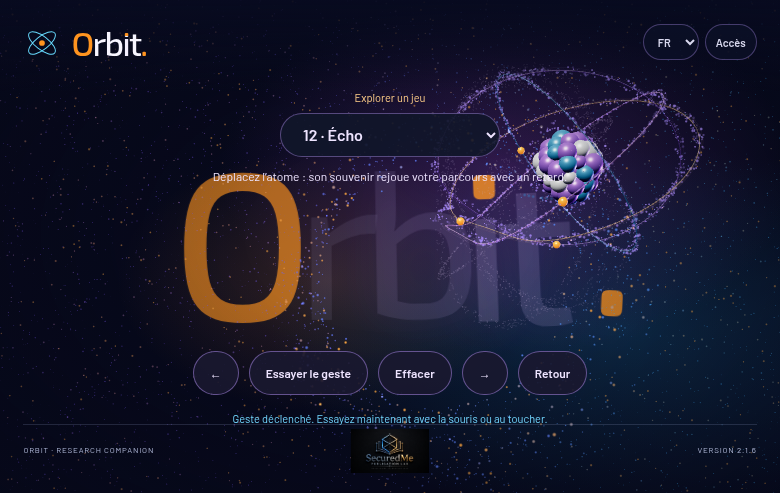
\includegraphics[keepaspectratio,alt={Écho : état obtenu par la démonstration sur le domaine public, navigateur E2B piloté depuis Kaggle.}]{figures/echo.png}}
\caption{Écho : état obtenu par la démonstration sur le domaine public,
navigateur E2B piloté depuis Kaggle.}
\end{figure}

\subsubsection{Comprendre avant de
calculer}\label{comprendre-avant-de-calculer-11}

Une copie immédiate suivrait chaque mouvement. Un écho consulte des
états plus anciens. Il faut donc conserver positions, rotations et
temps, puis choisir une entrée située près du temps demandé.

\subsubsection{Le mécanisme et un
exemple}\label{le-muxe9canisme-et-un-exemple-11}

Chaque frame mobile ajoute un instantané ; la file conserve au maximum
240 entrées. Le fantôme prend la première entrée dont le temps est au
moins age − 1,5. La cadence et la durée réellement disponibles dépendent
du rendu. À 60 frames par seconde, 240 entrées représentent environ
quatre secondes. Le matériau du fantôme a une opacité de 0,15.

\subsubsection{Retrouver le code}\label{retrouver-le-code-11}

Extrait réel : \texttt{web/src/lib/atom-playground.ts}, ligne 229 dans
l'instantané de cette édition. Les retours à la ligne ont été ajoutés
après les points-virgules pour la lecture ; les instructions sont
conservées. Retrouvez aussi le marqueur
\texttt{histories.find(h=\textgreater{}h.time\textgreater{}=age-1.5)} si
les lignes ont changé.

\begin{Shaded}
\begin{Highlighting}[]
\ControlFlowTok{if}\NormalTok{(mode}\OperatorTok{===}\StringTok{\textquotesingle{}echo\textquotesingle{}}\NormalTok{)\{}\KeywordTok{const}\NormalTok{ entry}\OperatorTok{=}\NormalTok{histories}\OperatorTok{.}\FunctionTok{find}\NormalTok{(h}\KeywordTok{=\textgreater{}}\NormalTok{h}\OperatorTok{.}\AttributeTok{time}\OperatorTok{\textgreater{}=}\NormalTok{age}\OperatorTok{{-}}\FloatTok{1.5}\NormalTok{)}\OperatorTok{;}
\NormalTok{ghost}\OperatorTok{.}\AttributeTok{visible}\OperatorTok{=!!}\NormalTok{entry}\OperatorTok{;}
\ControlFlowTok{if}\NormalTok{(entry)\{ghost}\OperatorTok{.}\AttributeTok{position}\OperatorTok{.}\FunctionTok{copy}\NormalTok{(entry}\OperatorTok{.}\AttributeTok{position}\NormalTok{)}\OperatorTok{;}
\NormalTok{ghost}\OperatorTok{.}\AttributeTok{rotation}\OperatorTok{.}\FunctionTok{set}\NormalTok{(entry}\OperatorTok{.}\AttributeTok{x}\OperatorTok{,}\NormalTok{entry}\OperatorTok{.}\AttributeTok{y}\OperatorTok{,{-}.}\DecValTok{1}\NormalTok{)}\OperatorTok{;}
\NormalTok{ghost}\OperatorTok{.}\AttributeTok{scale}\OperatorTok{.}\FunctionTok{copy}\NormalTok{(c}\OperatorTok{.}\AttributeTok{atom}\OperatorTok{.}\AttributeTok{scale}\NormalTok{)}\OperatorTok{;}
\ControlFlowTok{if}\NormalTok{(moving)}\FunctionTok{emit}\NormalTok{(entry}\OperatorTok{.}\AttributeTok{position}\OperatorTok{,.}\DecValTok{3}\NormalTok{)}\OperatorTok{;}
\NormalTok{\}\}}
\end{Highlighting}
\end{Shaded}

\subsubsection{Vérifier et comprendre la
portée}\label{vuxe9rifier-et-comprendre-la-portuxe9e-11}

Le début de jeu n'a pas encore tout l'historique nécessaire. L'entrée
est choisie parmi des échantillons, sans interpolation temporelle fine.
La démonstration peut fabriquer un parcours explicatif ; votre geste
constitue un parcours différent. Le souvenir est une silhouette de
points ; il ne copie pas toutes les sphères éclairées et reste absent du
landing par défaut.

La validation cloud a contrôlé un signal de l'effet et l'absence de
valeur non finie après un geste natif. La capture ci-dessus montre un
état rendu. Cette combinaison protège un parcours précis ; votre essai
manuel vérifie aussi la sensation et la compréhension du geste. Le
bouton de démonstration constitue une aide, distincte d'une réalisation
autonome.

\subsubsection{Exercice à faire dans une copie de
développement}\label{exercice-uxe0-faire-dans-une-copie-de-duxe9veloppement-11}

Changez 1,5 en 0,75. Préparez un trajet avec un arrêt net et comparez le
décalage, en conservant 240 entrées. Avant d'exécuter, écrivez votre
prédiction. Après l'essai, relevez ce que vous avez observé et une
limite. Les pistes de correction sont regroupées à la fin du manuel.

\subsection{17. Remonter le temps --- Instantanés, restauration et
branche
d'historique}\label{remonter-le-temps-instantanuxe9s-restauration-et-branche-dhistorique}

\textbf{Geste.} Créez un parcours, puis maintenez sur le fond, loin du
noyau, pour rembobiner. Relâchez et créez un nouveau trajet à partir de
l'état retrouvé.

\begin{figure}
\centering
\pandocbounded{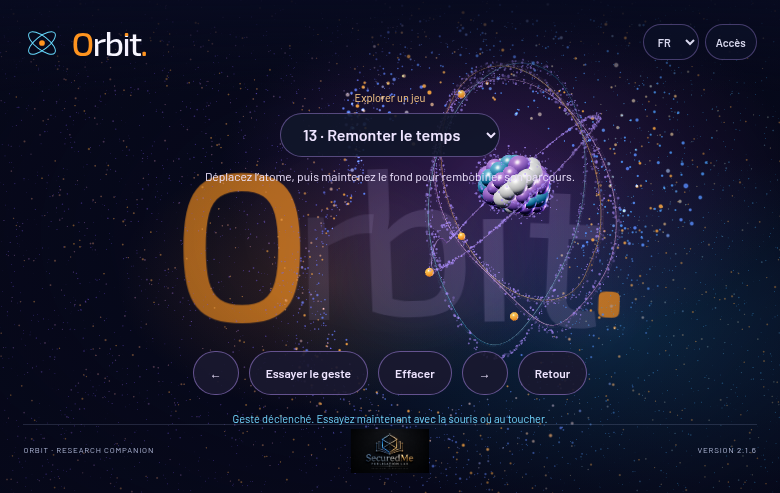
\includegraphics[keepaspectratio,alt={Remonter le temps : état obtenu par la démonstration sur le domaine public, navigateur E2B piloté depuis Kaggle.}]{figures/rewind.png}}
\caption{Remonter le temps : état obtenu par la démonstration sur le
domaine public, navigateur E2B piloté depuis Kaggle.}
\end{figure}

\subsubsection{Comprendre avant de
calculer}\label{comprendre-avant-de-calculer-12}

Le retour dans le temps d'une interface consiste à restaurer des données
enregistrées. Il ne remonte pas le temps réel : il relit une suite de
positions et de traces. Après un retour, un nouveau geste forme une
nouvelle branche et l'ancien futur est retiré.

\subsubsection{Le mécanisme et un
exemple}\label{le-muxe9canisme-et-un-exemple-12}

L'historique garde position, rotation, temps de scène, tableau de
positions du ruban et vies des points. rewindIndex part de la dernière
entrée, puis diminue de 60Δt. L'évaluation restaure les tableaux, remet
la vitesse à zéro et ajuste le déplacement. À la libération, splice
retire les entrées situées après la position courante. Les 240
instantanés sont une borne en nombre, pas en secondes.

\subsubsection{Retrouver le code}\label{retrouver-le-code-12}

Extrait réel : \texttt{web/src/lib/atom-playground.ts}, ligne 171 dans
l'instantané de cette édition. Les retours à la ligne ont été ajoutés
après les points-virgules pour la lecture ; les instructions sont
conservées. Retrouvez aussi le marqueur
\texttt{histories.splice(Math.max} si les lignes ont changé.

\begin{Shaded}
\begin{Highlighting}[]
\KeywordTok{function} \FunctionTok{finishRewind}\NormalTok{()\{}\ControlFlowTok{if}\NormalTok{(rewindIndex}\OperatorTok{\textgreater{}=}\DecValTok{0}\NormalTok{)histories}\OperatorTok{.}\FunctionTok{splice}\NormalTok{(}\BuiltInTok{Math}\OperatorTok{.}\FunctionTok{max}\NormalTok{(}\DecValTok{0}\OperatorTok{,}\BuiltInTok{Math}\OperatorTok{.}\FunctionTok{floor}\NormalTok{(rewindIndex)}\OperatorTok{+}\DecValTok{1}\NormalTok{))}\OperatorTok{;}
\NormalTok{rewindIndex}\OperatorTok{={-}}\DecValTok{1}\OperatorTok{;}
\NormalTok{held}\OperatorTok{=}\KeywordTok{false}\OperatorTok{;}
\NormalTok{\}}
\end{Highlighting}
\end{Shaded}

\subsubsection{Vérifier et comprendre la
portée}\label{vuxe9rifier-et-comprendre-la-portuxe9e-12}

Le retour restaure les données prévues pour ce mode, pas l'intégralité
de la scène, des menus ou du navigateur. La poussière et les gestes
futurs ne forment pas un moteur général d'annulation. Les copies de
tableaux rendent ce mode plus gourmand que l'écho simple.

La validation cloud a contrôlé un signal de l'effet et l'absence de
valeur non finie après un geste natif. La capture ci-dessus montre un
état rendu. Cette combinaison protège un parcours précis ; votre essai
manuel vérifie aussi la sensation et la compréhension du geste. Le
bouton de démonstration constitue une aide, distincte d'une réalisation
autonome.

\subsubsection{Exercice à faire dans une copie de
développement}\label{exercice-uxe0-faire-dans-une-copie-de-duxe9veloppement-12}

Comparez une vitesse de lecture de 60Δt et 30Δt. Décrivez la durée du
retour pour un même historique. Avant d'exécuter, écrivez votre
prédiction. Après l'essai, relevez ce que vous avez observé et une
limite. Les pistes de correction sont regroupées à la fin du manuel.

\subsection{18. Rencontre --- Distance et relation
visuelle}\label{rencontre-distance-et-relation-visuelle}

\textbf{Geste.} Approchez le noyau du petit compagnon. Une tresse
lumineuse relie les deux, et deux flux parcourent la liaison.

\begin{figure}
\centering
\pandocbounded{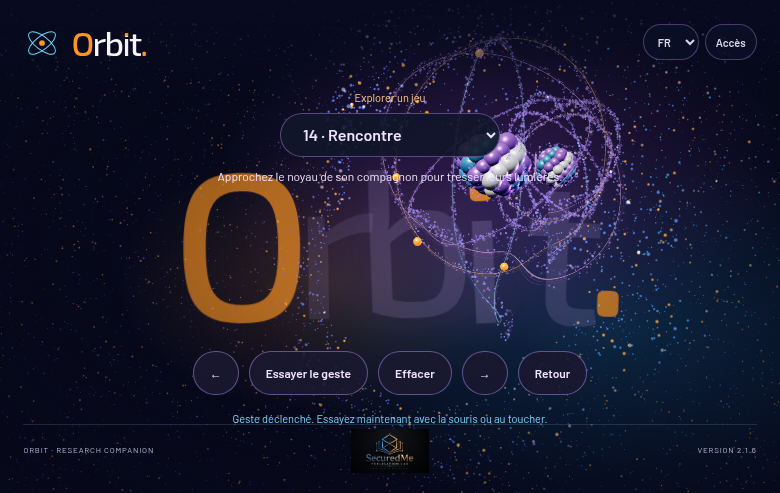
\includegraphics[keepaspectratio,alt={Rencontre : état obtenu par la démonstration sur le domaine public, navigateur E2B piloté depuis Kaggle.}]{figures/duet.png}}
\caption{Rencontre : état obtenu par la démonstration sur le domaine
public, navigateur E2B piloté depuis Kaggle.}
\end{figure}

\subsubsection{Comprendre avant de
calculer}\label{comprendre-avant-de-calculer-13}

La présence d'une liaison dépend de la proximité. La tresse n'a pas
besoin d'être un objet rigide : elle peut être reconstruite à partir de
positions entre deux extrémités. Un motif sinusoïdal lui donne son
apparence.

\subsubsection{Le mécanisme et un
exemple}\label{le-muxe9canisme-et-un-exemple-13}

connection = max(0,1 − distance/4). À deux unités de distance, la valeur
est 0,5 ; au-delà de quatre, elle vaut zéro. Les 96 points de la ligne
interpolent entre les deux atomes ; des sinus et cosinus ajoutent un
décalage de 0,22 × connection. Des particules traversent dans les deux
sens si connection dépasse 0,5. Le compagnon mesure 40 \% de l'échelle
de référence du clone.

\subsubsection{Retrouver le code}\label{retrouver-le-code-13}

Extrait réel : \texttt{web/src/lib/atom-playground.ts}, ligne 231 dans
l'instantané de cette édition. Les retours à la ligne ont été ajoutés
après les points-virgules pour la lecture ; les instructions sont
conservées. Retrouvez aussi le marqueur
\texttt{connection=Math.max(0,1-distance/4)} si les lignes ont changé.

\begin{Shaded}
\begin{Highlighting}[]
\ControlFlowTok{if}\NormalTok{(mode}\OperatorTok{===}\StringTok{\textquotesingle{}duet\textquotesingle{}}\NormalTok{)\{duet}\OperatorTok{.}\AttributeTok{rotation}\OperatorTok{.}\FunctionTok{set}\NormalTok{(c}\OperatorTok{.}\AttributeTok{atom}\OperatorTok{.}\AttributeTok{rotation}\OperatorTok{.}\AttributeTok{x}\OperatorTok{,{-}}\NormalTok{c}\OperatorTok{.}\AttributeTok{atom}\OperatorTok{.}\AttributeTok{rotation}\OperatorTok{.}\AttributeTok{y}\OperatorTok{,}\DecValTok{0}\NormalTok{)}\OperatorTok{;}
\KeywordTok{const}\NormalTok{ distance}\OperatorTok{=}\NormalTok{atomPosition}\OperatorTok{.}\FunctionTok{distanceTo}\NormalTok{(duetPosition)}\OperatorTok{;}
\KeywordTok{const}\NormalTok{ connection}\OperatorTok{=}\BuiltInTok{Math}\OperatorTok{.}\FunctionTok{max}\NormalTok{(}\DecValTok{0}\OperatorTok{,}\DecValTok{1}\OperatorTok{{-}}\NormalTok{distance}\OperatorTok{/}\DecValTok{4}\NormalTok{)}\OperatorTok{;}
\NormalTok{braid}\OperatorTok{.}\AttributeTok{visible}\OperatorTok{=}\NormalTok{connection}\OperatorTok{\textgreater{}.}\BaseNTok{01}\OperatorTok{;}
\ControlFlowTok{for}\NormalTok{(}\KeywordTok{let}\NormalTok{ i}\OperatorTok{=}\DecValTok{0}\OperatorTok{;}
\NormalTok{i}\OperatorTok{\textless{}}\DecValTok{96}\OperatorTok{;}
\NormalTok{i}\OperatorTok{++}\NormalTok{)\{}\KeywordTok{const}\NormalTok{ t}\OperatorTok{=}\NormalTok{i}\OperatorTok{/}\DecValTok{95}\OperatorTok{,}\NormalTok{p}\OperatorTok{=}\NormalTok{atomPosition}\OperatorTok{.}\FunctionTok{clone}\NormalTok{()}\OperatorTok{.}\FunctionTok{lerp}\NormalTok{(duetPosition}\OperatorTok{,}\NormalTok{t)}\OperatorTok{;}
\NormalTok{p}\OperatorTok{.}\AttributeTok{y}\OperatorTok{+=}\BuiltInTok{Math}\OperatorTok{.}\FunctionTok{sin}\NormalTok{(t}\OperatorTok{*}\BuiltInTok{Math}\OperatorTok{.}\ConstantTok{PI}\OperatorTok{*}\DecValTok{12}\OperatorTok{+}\NormalTok{age}\OperatorTok{*}\DecValTok{3}\NormalTok{)}\OperatorTok{*.}\DecValTok{22}\OperatorTok{*}\NormalTok{connection}\OperatorTok{;}
\NormalTok{p}\OperatorTok{.}\AttributeTok{z}\OperatorTok{+=}\BuiltInTok{Math}\OperatorTok{.}\FunctionTok{cos}\NormalTok{(t}\OperatorTok{*}\BuiltInTok{Math}\OperatorTok{.}\ConstantTok{PI}\OperatorTok{*}\DecValTok{12}\OperatorTok{+}\NormalTok{age}\OperatorTok{*}\DecValTok{3}\NormalTok{)}\OperatorTok{*.}\DecValTok{22}\OperatorTok{*}\NormalTok{connection}\OperatorTok{;}
\NormalTok{p}\OperatorTok{.}\FunctionTok{toArray}\NormalTok{(braidArray}\OperatorTok{,}\NormalTok{i}\OperatorTok{*}\DecValTok{3}\NormalTok{)}\OperatorTok{;}
\NormalTok{\}braidGeometry}\OperatorTok{.}\AttributeTok{attributes}\OperatorTok{.}\AttributeTok{position}\OperatorTok{.}\AttributeTok{needsUpdate}\OperatorTok{=}\KeywordTok{true}\OperatorTok{;}
\ControlFlowTok{if}\NormalTok{(moving}\OperatorTok{\&\&}\NormalTok{connection}\OperatorTok{\textgreater{}.}\DecValTok{5}\NormalTok{)\{}\KeywordTok{const}\NormalTok{ t}\OperatorTok{=}\NormalTok{(age}\OperatorTok{*.}\DecValTok{45}\NormalTok{)}\OperatorTok{\%}\DecValTok{1}\OperatorTok{;}
\FunctionTok{emit}\NormalTok{(atomPosition}\OperatorTok{.}\FunctionTok{clone}\NormalTok{()}\OperatorTok{.}\FunctionTok{lerp}\NormalTok{(duetPosition}\OperatorTok{,}\NormalTok{t))}\OperatorTok{;}
\FunctionTok{emit}\NormalTok{(duetPosition}\OperatorTok{.}\FunctionTok{clone}\NormalTok{()}\OperatorTok{.}\FunctionTok{lerp}\NormalTok{(atomPosition}\OperatorTok{,}\NormalTok{t))}\OperatorTok{;}
\NormalTok{\}\}}
\end{Highlighting}
\end{Shaded}

\subsubsection{Vérifier et comprendre la
portée}\label{vuxe9rifier-et-comprendre-la-portuxe9e-13}

Il s'agit d'une relation graphique déclenchée par la distance. Aucun
échange de messages, transfert d'énergie ou synchronisation scientifique
entre atomes n'est calculé. Le petit compagnon a une position fixe.

La validation cloud a contrôlé un signal de l'effet et l'absence de
valeur non finie après un geste natif. La capture ci-dessus montre un
état rendu. Cette combinaison protège un parcours précis ; votre essai
manuel vérifie aussi la sensation et la compréhension du geste. Le
bouton de démonstration constitue une aide, distincte d'une réalisation
autonome.

\subsubsection{Exercice à faire dans une copie de
développement}\label{exercice-uxe0-faire-dans-une-copie-de-duxe9veloppement-13}

Changez le rayon de relation 4 en 3. Prédisez où la tresse disparaîtra.
Gardez séparément le seuil d'émission de 0,5. Avant d'exécuter, écrivez
votre prédiction. Après l'essai, relevez ce que vous avez observé et une
limite. Les pistes de correction sont regroupées à la fin du manuel.

\subsection{19. Empreinte --- Composition d'image et export
local}\label{empreinte-composition-dimage-et-export-local}

\textbf{Geste.} Composez votre scène, puis choisissez Empreinte et
Enregistrer PNG. Le navigateur prépare une image à télécharger sur votre
appareil.

\begin{figure}
\centering
\pandocbounded{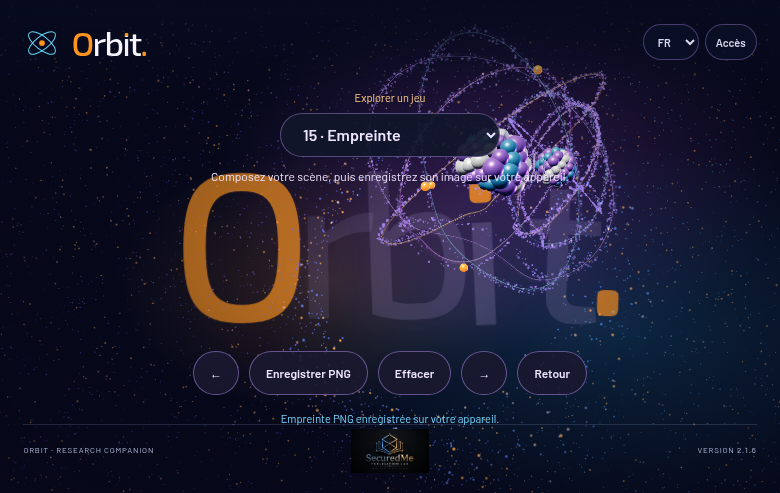
\includegraphics[keepaspectratio,alt={Empreinte : état obtenu par la démonstration sur le domaine public, navigateur E2B piloté depuis Kaggle.}]{figures/capture.png}}
\caption{Empreinte : état obtenu par la démonstration sur le domaine
public, navigateur E2B piloté depuis Kaggle.}
\end{figure}

\subsubsection{Comprendre avant de
calculer}\label{comprendre-avant-de-calculer-14}

La capture transforme une scène interactive en document fixe. Le
programme dessine d'abord la scène, puis la copie sur un second canvas,
ajoute le fond et le mot Orbit si nécessaire, et produit un fichier PNG.

\subsubsection{Le mécanisme et un
exemple}\label{le-muxe9canisme-et-un-exemple-14}

renderer.render précède drawImage. Le canvas de sortie reprend les
dimensions réelles du canvas WebGL. Son fond vaut \#080b20 ; la mise à
l'échelle permet d'ajouter les lettres selon leur position dans la page.
toBlob produit le PNG de manière asynchrone. Une URL temporaire
déclenche le téléchargement, puis URL.revokeObjectURL la libère après
une seconde.

\subsubsection{Retrouver le code}\label{retrouver-le-code-14}

Extrait réel : \texttt{web/src/lib/atom-playground.ts}, ligne 145 dans
l'instantané de cette édition. Les retours à la ligne ont été ajoutés
après les points-virgules pour la lecture ; les instructions sont
conservées. Retrouvez aussi le marqueur
\texttt{image.toBlob(blob=\textgreater{}} si les lignes ont changé.

\begin{Shaded}
\begin{Highlighting}[]
\NormalTok{image}\OperatorTok{.}\FunctionTok{toBlob}\NormalTok{(blob}\KeywordTok{=\textgreater{}}\NormalTok{\{}\ControlFlowTok{if}\NormalTok{(}\OperatorTok{!}\NormalTok{blob)\{}\FunctionTok{message}\NormalTok{(}\StringTok{\textquotesingle{}Capture indisponible. Réessayez.\textquotesingle{}}\NormalTok{)}\OperatorTok{;}
\ControlFlowTok{return}\OperatorTok{;}
\NormalTok{\}captures}\OperatorTok{++;}
\NormalTok{c}\OperatorTok{.}\AttributeTok{scope}\OperatorTok{.}\AttributeTok{dataset}\OperatorTok{.}\AttributeTok{gameCaptures}\OperatorTok{=}\BuiltInTok{String}\NormalTok{(captures)}\OperatorTok{;}
\KeywordTok{const}\NormalTok{ url}\OperatorTok{=}\NormalTok{URL}\OperatorTok{.}\FunctionTok{createObjectURL}\NormalTok{(blob)}\OperatorTok{;}
\KeywordTok{const}\NormalTok{ link}\OperatorTok{=}\BuiltInTok{document}\OperatorTok{.}\FunctionTok{createElement}\NormalTok{(}\StringTok{\textquotesingle{}a\textquotesingle{}}\NormalTok{)}\OperatorTok{;}
\NormalTok{link}\OperatorTok{.}\AttributeTok{href}\OperatorTok{=}\NormalTok{url}\OperatorTok{;}
\NormalTok{link}\OperatorTok{.}\AttributeTok{download}\OperatorTok{=}\StringTok{\textquotesingle{}orbit{-}empreinte.png\textquotesingle{}}\OperatorTok{;}
\NormalTok{link}\OperatorTok{.}\FunctionTok{click}\NormalTok{()}\OperatorTok{;}
\PreprocessorTok{setTimeout}\NormalTok{(()}\KeywordTok{=\textgreater{}}\NormalTok{URL}\OperatorTok{.}\FunctionTok{revokeObjectURL}\NormalTok{(url)}\OperatorTok{,}\DecValTok{1000}\NormalTok{)}\OperatorTok{;}
\FunctionTok{message}\NormalTok{(}\StringTok{\textquotesingle{}Empreinte PNG enregistrée sur votre appareil.\textquotesingle{}}\NormalTok{)}\OperatorTok{;}
\NormalTok{\}}\OperatorTok{,}\StringTok{\textquotesingle{}image/png\textquotesingle{}}\NormalTok{)}\OperatorTok{;}
\end{Highlighting}
\end{Shaded}

\subsubsection{Vérifier et comprendre la
portée}\label{vuxe9rifier-et-comprendre-la-portuxe9e-14}

L'image représente la composition de scène, pas une capture intégrale
des contrôles HTML. Le téléchargement peut dépendre des règles du
navigateur. Un PNG conserve des pixels ; il ne permet pas de reprendre
l'état interactif. Aucune image n'est envoyée à un serveur par ce jeu.

La validation cloud a contrôlé un signal de l'effet et l'absence de
valeur non finie après un geste natif. La capture ci-dessus montre un
état rendu. Cette combinaison protège un parcours précis ; votre essai
manuel vérifie aussi la sensation et la compréhension du geste. Le
bouton de démonstration constitue une aide, distincte d'une réalisation
autonome.

\subsubsection{Exercice à faire dans une copie de
développement}\label{exercice-uxe0-faire-dans-une-copie-de-duxe9veloppement-14}

Remplacez seulement la légende ma constellation par un titre court de
votre atelier. Vérifiez la lisibilité et restaurez la version du projet
avant une livraison publique. Avant d'exécuter, écrivez votre
prédiction. Après l'essai, relevez ce que vous avez observé et une
limite. Les pistes de correction sont regroupées à la fin du manuel.

\subsection{20. Rendre l'expérience
fiable}\label{rendre-lexpuxe9rience-fiable}

Chaque jeu utilise un stock borné : 32 étoiles, 128 points de couronne,
1 024 points de ruban, 240 états d'historique, 96 points pour la tresse.
Les limites sont des décisions de conception. Les jeux temporels
conservent des tableaux de trace. Le landing n'enregistre aucun
historique automatique. Les 55 sphères gardent leurs transformations
indépendantes, mais sont dessinées par quatre groupes InstancedMesh de
même matériau ; cela réduit les appels de dessin sans changer leur
identité visuelle. Le jeu Écho utilise désormais une silhouette de
points en une seule commande de dessin, au lieu d'une copie de tous les
maillages éclairés. Une optimisation utile commence par observer
allocations et temps de frame sur un appareil représentatif, pas par
diminuer toutes les capacités arbitrairement.

Le playground possède son AbortController. Lors du nettoyage, il enlève
ses événements et son panneau, retire son groupe de la scène, libère ses
géométries propres et ses matériaux. Les clones partagent certaines
géométries du noyau : ce partage doit être respecté pour ne pas détruire
un objet encore utilisé. La scène principale arrête son rendu et libère
ensuite ses ressources. Les contrôles cloud n'ont pas mesuré
exhaustivement une fuite après cent transitions ; ce point reste un
contrôle complémentaire possible.

Le menu Accès reste sombre et simple. Statique fige la scène actuelle ;
les objets ne sont pas supprimés et le canvas reste visible. Reprendre
réactive la même scène. Le contraste renforcé et le texte agrandi sont
des préférences locales, conservées avec la langue FR/EN/ES sous un
contrat commun versionné. Le nom Orbit. reste non traduisible ; le O
majuscule, les points et le point du i utilisent l'accent orange. Le
mouvement réduit du système bloque ou fige certaines animations
automatiques et conserve les commandes de démonstration adaptées. La
pause agit sur le temps du rendu. En cas de perte de contexte WebGL, la
scène rend la navigation ordinaire et l'illustration statique
accessibles. L'absence de WebGL signifie que les jeux 3D ne sont pas
disponibles ; elle ne signifie pas que l'utilisateur est empêché
d'ouvrir Orbit, Studio ou Documentation.

Sur petit écran, le sélecteur et les boutons restent dans une largeur
disponible. Le contrôle automatique couvre un format de 390 × 844 pixels
; il ne remplace pas l'observation sur tous les appareils. Pour faire
évoluer le code, changez un paramètre à la fois, gardez le geste
comparable, notez les différences et restaurez la valeur avant une autre
expérience.

\subsection{21. Votre journal de
compréhension}\label{votre-journal-de-compruxe9hension}

Complétez les lignes avec des observations datées. Une réponse que vous
pouvez expliquer et transférer est plus utile qu'un score de jeu.

{\def\LTcaptype{none} % do not increment counter
\begin{longtable}[]{@{}
  >{\raggedright\arraybackslash}p{(\linewidth - 8\tabcolsep) * \real{0.2000}}
  >{\raggedright\arraybackslash}p{(\linewidth - 8\tabcolsep) * \real{0.2000}}
  >{\raggedright\arraybackslash}p{(\linewidth - 8\tabcolsep) * \real{0.2000}}
  >{\raggedright\arraybackslash}p{(\linewidth - 8\tabcolsep) * \real{0.2000}}
  >{\raggedright\arraybackslash}p{(\linewidth - 8\tabcolsep) * \real{0.2000}}@{}}
\toprule\noalign{}
\begin{minipage}[b]{\linewidth}\raggedright
Notion
\end{minipage} & \begin{minipage}[b]{\linewidth}\raggedright
Rencontrée dans
\end{minipage} & \begin{minipage}[b]{\linewidth}\raggedright
Mon essai
\end{minipage} & \begin{minipage}[b]{\linewidth}\raggedright
Ce que je peux expliquer
\end{minipage} & \begin{minipage}[b]{\linewidth}\raggedright
Nouvelle application
\end{minipage} \\
\midrule\noalign{}
\endhead
\bottomrule\noalign{}
\endlastfoot
Position / vitesse & Fronde, lancer & À compléter & À compléter & À
compléter \\
Amortissement & Élastique, rebond & À compléter & À compléter & À
compléter \\
Interpolation & Vortex, Rencontre & À compléter & À compléter & À
compléter \\
Stock borné & Pinceau, Écho & À compléter & À compléter & À compléter \\
État / événement & Portails, retour & À compléter & À compléter & À
compléter \\
Export & Empreinte & À compléter & À compléter & À compléter \\
\end{longtable}
}

\textbf{Bilan à la première personne, à compléter :} « J'ai
observé\ldots{} Mon hypothèse était\ldots{} Dans le code, le
paramètre\ldots{} Cette expérience montre\ldots{} La limite de mon
observation est\ldots{} Pour vérifier mon explication, je peux
essayer\ldots{} »

\section{Partie II --- apprendre à
l'enseigner}\label{partie-ii-apprendre-uxe0-lenseigner}

\subsection{22. Une méthode pour chaque
rencontre}\label{une-muxe9thode-pour-chaque-rencontre}

Commencez par un effet visible. Laissez l'étudiant prédire avant le clic
ou la modification. Expliquez une idée, montrez le petit morceau de code
qui la réalise, puis laissez une expérience réversible. Demandez une
reformulation et une application nouvelle. Votre rôle consiste à
organiser cette progression ; le logiciel n'observe pas automatiquement
la compréhension.

Les activités suivantes sont des propositions à réaliser avec un
étudiant. Les résultats attendus restent des pistes, pas des témoignages
d'un atelier déjà effectué. Adaptez vocabulaire, nombres et durée à son
aisance avec coordonnées et programmation. Un débutant peut travailler
sur papier et dans le site ; un étudiant plus avancé peut modifier une
copie de code. Le matériel est une machine avec navigateur, une feuille
et un crayon. La ficelle de l'activité Cordes est facultative.

Pour chaque activité, consacrez environ deux minutes à montrer et
prédire, trois à cinq minutes à expérimenter, puis deux minutes à
expliquer et transférer. Cette durée est une estimation pédagogique, à
ajuster à la personne. L'étudiant gagne du temps de réflexion ;
l'enseignant évite de remplir immédiatement chaque silence.

\subsection{23. Parler avec votre
intention}\label{parler-avec-votre-intention}

Les scripts proposés gardent l'enthousiasme du projet : une expérience
visible, une hypothèse, un essai et une explication reliée au code. Ils
utilisent une première personne de démonstration, par exemple « Je vais
essayer\ldots{} » ou « Mon hypothèse est\ldots{} ». Les pauses et
intonations sont des indications de lecture. Aucun enregistrement de
référence n'a servi à reproduire votre voix réelle.

\textbf{{[}Pause{]}} laisse le temps d'observer. \textbf{{[}Accent{]}}
souligne la conséquence. \textbf{{[}Ralentir{]}} accompagne un terme
nouveau. \textbf{{[}Énergie{]}} accompagne le geste, sans remplacer
l'explication. Évitez d'annoncer « tu as compris » après un succès :
demandez plutôt ce qui permettait de le prédire.

\subsection{Activité 01 --- Le défi de la cible
invisible}\label{activituxe9-01-le-duxe9fi-de-la-cible-invisible}

\textbf{Jeu : Fronde. Objectif :} Distinguer distance, direction et
vitesse, en observant un geste identique deux fois.

\textbf{Préparation.} Ouvrez le jeu, utilisez Effacer lorsque c'est
pertinent, puis faites un seul geste de démonstration. Expliquez que
l'essai de l'étudiant vient ensuite. Préparez une feuille pour noter sa
prédiction et son observation. Les modifications de code se font dans
une copie réversible.

\textbf{Question avant l'action :} Si je tire à droite du noyau, dans
quel sens la perle part-elle ? Un étirement deux fois plus grand
donne-t-il toujours deux fois plus de vitesse ?

\subsubsection{Déroulement avec
l'étudiant}\label{duxe9roulement-avec-luxe9tudiant}

\begin{enumerate}
\def\labelenumi{\arabic{enumi}.}
\tightlist
\item
  Dessinez sur une feuille le noyau et deux positions de départ à
  droite. Faites tracer la flèche attendue avant de toucher l'écran.
\item
  L'étudiant tire peu, relâche, puis recommence avec un étirement plus
  grand. Il note le sens et la longueur visible du trajet, pas une
  vitesse prétendument mesurée.
\item
  Inversez les rôles : l'étudiant annonce un geste, vous prédisez le
  mouvement. Examinez ensemble le plafond et le rebond.
\item
  Dans la copie de code, essayez le coefficient 2. Comparez à
  l'hypothèse, puis restaurez 3.
\end{enumerate}

\subsubsection{Une entrée orale
proposée}\label{une-entruxe9e-orale-proposuxe9e}

« {[}Énergie{]} On va partir de quelque chose qu'on peut vraiment
manipuler. {[}Pause{]} Mon hypothèse, je l'écris avant d'essayer. Pour
fronde, si je tire à droite du noyau, dans quel sens la perle part-elle
? Un étirement deux fois plus grand donne-t-il toujours deux fois plus
de vitesse ? {[}Ralentir{]} Après le geste, on cherchera la donnée du
programme qui explique le résultat. Si notre observation diffère, on
garde la différence : elle nous aide à trouver ce qu'on avait oublié. »

\subsubsection{Vérifier la
compréhension}\label{vuxe9rifier-la-compruxe9hension}

Demandez à l'étudiant de raconter le mécanisme sans lire le chapitre.
Faites-lui nommer un paramètre, son rôle et une limite. Une bonne
reformulation distingue ce qu'il a vu et ce qu'il suppose. Pour une
vérification de transfert, demandez : \textbf{Comment utiliseriez-vous
position et vitesse pour faire glisser une carte de jeu ?}

\textbf{Trace de l'atelier.} Prédiction : \_\_\_\_\_\_. Observation :
\_\_\_\_\_\_. Explication de l'étudiant : \_\_\_\_\_\_. Ce qui reste à
clarifier : \_\_\_\_\_\_. Date et version essayée : \_\_\_\_\_\_.

\subsection{Activité 02 --- Le dessin qui
s'oublie}\label{activituxe9-02-le-dessin-qui-soublie}

\textbf{Jeu : Pinceau. Objectif :} Comprendre pourquoi une limite de
mémoire peut être compatible avec une trace continue.

\textbf{Préparation.} Ouvrez le jeu, utilisez Effacer lorsque c'est
pertinent, puis faites un seul geste de démonstration. Expliquez que
l'essai de l'étudiant vient ensuite. Préparez une feuille pour noter sa
prédiction et son observation. Les modifications de code se font dans
une copie réversible.

\textbf{Question avant l'action :} Que devient le premier point si nous
dessinons plus longtemps que la capacité du tableau ?

\subsubsection{Déroulement avec
l'étudiant}\label{duxe9roulement-avec-luxe9tudiant-1}

\begin{enumerate}
\def\labelenumi{\arabic{enumi}.}
\tightlist
\item
  Faites tracer un huit avec le noyau ; demandez à l'étudiant de
  désigner la partie la plus ancienne.
\item
  Attendez en observant la disparition, puis dessinez à nouveau.
  L'étudiant distingue création et extinction.
\item
  Sur une feuille, numérotez huit cases : écrivez une position dans
  chacune, puis revenez à la première. Ce petit modèle représente le
  buffer de 1 024 cases.
\item
  Modifiez seulement la vitesse d'extinction dans la copie de
  développement et comparez deux essais.
\end{enumerate}

\subsubsection{Une entrée orale
proposée}\label{une-entruxe9e-orale-proposuxe9e-1}

« {[}Énergie{]} On va partir de quelque chose qu'on peut vraiment
manipuler. {[}Pause{]} Mon hypothèse, je l'écris avant d'essayer. Pour
pinceau, que devient le premier point si nous dessinons plus longtemps
que la capacité du tableau ? {[}Ralentir{]} Après le geste, on cherchera
la donnée du programme qui explique le résultat. Si notre observation
diffère, on garde la différence : elle nous aide à trouver ce qu'on
avait oublié. »

\subsubsection{Vérifier la
compréhension}\label{vuxe9rifier-la-compruxe9hension-1}

Demandez à l'étudiant de raconter le mécanisme sans lire le chapitre.
Faites-lui nommer un paramètre, son rôle et une limite. Une bonne
reformulation distingue ce qu'il a vu et ce qu'il suppose. Pour une
vérification de transfert, demandez : \textbf{Quel autre usage pourrait
avoir un stock circulaire : historique de capteur, journal limité,
dernières positions d'un personnage ?}

\textbf{Trace de l'atelier.} Prédiction : \_\_\_\_\_\_. Observation :
\_\_\_\_\_\_. Explication de l'étudiant : \_\_\_\_\_\_. Ce qui reste à
clarifier : \_\_\_\_\_\_. Date et version essayée : \_\_\_\_\_\_.

\subsection{Activité 03 --- La corde
humaine}\label{activituxe9-03-la-corde-humaine}

\textbf{Jeu : Cordes. Objectif :} Séparer amplitude, motif spatial et
évolution dans le temps.

\textbf{Préparation.} Ouvrez le jeu, utilisez Effacer lorsque c'est
pertinent, puis faites un seul geste de démonstration. Expliquez que
l'essai de l'étudiant vient ensuite. Préparez une feuille pour noter sa
prédiction et son observation. Les modifications de code se font dans
une copie réversible.

\textbf{Question avant l'action :} Si je tire plus loin, les bosses
deviennent-elles plus hautes ou plus nombreuses ?

\subsubsection{Déroulement avec
l'étudiant}\label{duxe9roulement-avec-luxe9tudiant-2}

\begin{enumerate}
\def\labelenumi{\arabic{enumi}.}
\tightlist
\item
  Deux personnes tiennent une ficelle légère. Produisez une petite puis
  une grande ondulation, sans changer volontairement la cadence.
\item
  Reproduisez deux amplitudes de geste dans Orbit. L'étudiant dessine le
  motif immédiatement après libération.
\item
  Examinez les facteurs 0,12, 5 et 8 : associez chacun à hauteur, motif
  ou évolution.
\item
  Dans le code, modifiez uniquement 5 en 3. Comparez les crêtes à votre
  dessin, puis restaurez la valeur.
\end{enumerate}

\subsubsection{Une entrée orale
proposée}\label{une-entruxe9e-orale-proposuxe9e-2}

« {[}Énergie{]} On va partir de quelque chose qu'on peut vraiment
manipuler. {[}Pause{]} Mon hypothèse, je l'écris avant d'essayer. Pour
cordes, si je tire plus loin, les bosses deviennent-elles plus hautes ou
plus nombreuses ? {[}Ralentir{]} Après le geste, on cherchera la donnée
du programme qui explique le résultat. Si notre observation diffère, on
garde la différence : elle nous aide à trouver ce qu'on avait oublié. »

\subsubsection{Vérifier la
compréhension}\label{vuxe9rifier-la-compruxe9hension-2}

Demandez à l'étudiant de raconter le mécanisme sans lire le chapitre.
Faites-lui nommer un paramètre, son rôle et une limite. Une bonne
reformulation distingue ce qu'il a vu et ce qu'il suppose. Pour une
vérification de transfert, demandez : \textbf{Comment dessineriez-vous
un drapeau qui ondule plus fort sans augmenter son nombre de plis ?}

\textbf{Trace de l'atelier.} Prédiction : \_\_\_\_\_\_. Observation :
\_\_\_\_\_\_. Explication de l'étudiant : \_\_\_\_\_\_. Ce qui reste à
clarifier : \_\_\_\_\_\_. Date et version essayée : \_\_\_\_\_\_.

\subsection{Activité 04 --- Le retour
tranquille}\label{activituxe9-04-le-retour-tranquille}

\textbf{Jeu : Élastique. Objectif :} Relier retour au repos et
dissipation, sans confondre les deux coefficients.

\textbf{Préparation.} Ouvrez le jeu, utilisez Effacer lorsque c'est
pertinent, puis faites un seul geste de démonstration. Expliquez que
l'essai de l'étudiant vient ensuite. Préparez une feuille pour noter sa
prédiction et son observation. Les modifications de code se font dans
une copie réversible.

\textbf{Question avant l'action :} Quel coefficient modifier pour calmer
le rebond tout en gardant la même attraction vers le repos ?

\subsubsection{Déroulement avec
l'étudiant}\label{duxe9roulement-avec-luxe9tudiant-3}

\begin{enumerate}
\def\labelenumi{\arabic{enumi}.}
\tightlist
\item
  Faites un étirement comparable deux fois. L'étudiant décrit ce qui
  revient et ce qui oscille.
\item
  Tracez trois cases sur papier : déformation, vitesse de retour, temps.
  Faites une seule étape numérique avec les valeurs du chapitre.
\item
  Essayez l'amortissement 6. L'étudiant observe le changement et compare
  à sa prédiction.
\item
  Il explique la différence entre un retour rapide, un rebond et une
  disparition instantanée.
\end{enumerate}

\subsubsection{Une entrée orale
proposée}\label{une-entruxe9e-orale-proposuxe9e-3}

« {[}Énergie{]} On va partir de quelque chose qu'on peut vraiment
manipuler. {[}Pause{]} Mon hypothèse, je l'écris avant d'essayer. Pour
élastique, quel coefficient modifier pour calmer le rebond tout en
gardant la même attraction vers le repos ? {[}Ralentir{]} Après le
geste, on cherchera la donnée du programme qui explique le résultat. Si
notre observation diffère, on garde la différence : elle nous aide à
trouver ce qu'on avait oublié. »

\subsubsection{Vérifier la
compréhension}\label{vuxe9rifier-la-compruxe9hension-3}

Demandez à l'étudiant de raconter le mécanisme sans lire le chapitre.
Faites-lui nommer un paramètre, son rôle et une limite. Une bonne
reformulation distingue ce qu'il a vu et ce qu'il suppose. Pour une
vérification de transfert, demandez : \textbf{Où utiliser un ressort
amorti dans une interface : bouton, panneau, caméra ou curseur ?}

\textbf{Trace de l'atelier.} Prédiction : \_\_\_\_\_\_. Observation :
\_\_\_\_\_\_. Explication de l'étudiant : \_\_\_\_\_\_. Ce qui reste à
clarifier : \_\_\_\_\_\_. Date et version essayée : \_\_\_\_\_\_.

\subsection{Activité 05 --- La carte du
tourbillon}\label{activituxe9-05-la-carte-du-tourbillon}

\textbf{Jeu : Vortex. Objectif :} Comprendre un effet local dont
l'intensité dépend de la distance.

\textbf{Préparation.} Ouvrez le jeu, utilisez Effacer lorsque c'est
pertinent, puis faites un seul geste de démonstration. Expliquez que
l'essai de l'étudiant vient ensuite. Préparez une feuille pour noter sa
prédiction et son observation. Les modifications de code se font dans
une copie réversible.

\textbf{Question avant l'action :} La poussière située loin du centre
devrait-elle tourner autant que celle située près ?

\subsubsection{Déroulement avec
l'étudiant}\label{duxe9roulement-avec-luxe9tudiant-4}

\begin{enumerate}
\def\labelenumi{\arabic{enumi}.}
\tightlist
\item
  Sur papier, dessinez trois cercles autour d'un centre. L'étudiant
  attribue qualitativement une influence forte, moyenne ou faible.
\item
  Dans Orbit, déplacez le centre lentement puis rapidement. Observez les
  zones les plus perturbées.
\item
  Calculez ensemble le premier pas d'interpolation de 0 vers 2. Faites
  ensuite un second pas : 0,3 + 0,15 × 1,7.
\item
  Essayez 0,4 dans la copie de code. L'étudiant compare le retard
  ressenti, puis explique la différence avec la force du tourbillon.
\item
  Sur le landing, chronométrez ensuite trois maintiens : 1,5 seconde,
  2,8 secondes, 4,5 secondes puis 6,8 secondes. Prédisez le seuil
  d'aspiration celui du logo ASCII puis celui de l'explosion ; relâchez
  et vérifiez la recomposition. Recommencez en mode Statique pour
  expliquer le rôle d'une garde d'entrée.
\end{enumerate}

\subsubsection{Une entrée orale
proposée}\label{une-entruxe9e-orale-proposuxe9e-4}

« {[}Énergie{]} On va partir de quelque chose qu'on peut vraiment
manipuler. {[}Pause{]} Mon hypothèse, je l'écris avant d'essayer. Pour
vortex, la poussière située loin du centre devrait-elle tourner autant
que celle située près ? {[}Ralentir{]} Après le geste, on cherchera la
donnée du programme qui explique le résultat. Si notre observation
diffère, on garde la différence : elle nous aide à trouver ce qu'on
avait oublié. »

\subsubsection{Vérifier la
compréhension}\label{vuxe9rifier-la-compruxe9hension-4}

Demandez à l'étudiant de raconter le mécanisme sans lire le chapitre.
Faites-lui nommer un paramètre, son rôle et une limite. Une bonne
reformulation distingue ce qu'il a vu et ce qu'il suppose. Pour une
vérification de transfert, demandez : \textbf{Comment faire suivre une
caméra à un objet tout en conservant un retard contrôlé ?}

\textbf{Trace de l'atelier.} Prédiction : \_\_\_\_\_\_. Observation :
\_\_\_\_\_\_. Explication de l'étudiant : \_\_\_\_\_\_. Ce qui reste à
clarifier : \_\_\_\_\_\_. Date et version essayée : \_\_\_\_\_\_.

\subsection{Activité 06 --- Le mot fait de
graines}\label{activituxe9-06-le-mot-fait-de-graines}

\textbf{Jeu : Sculpter Orbit. Objectif :} Relier une image en pixels à
une géométrie de points.

\textbf{Préparation.} Ouvrez le jeu, utilisez Effacer lorsque c'est
pertinent, puis faites un seul geste de démonstration. Expliquez que
l'essai de l'étudiant vient ensuite. Préparez une feuille pour noter sa
prédiction et son observation. Les modifications de code se font dans
une copie réversible.

\textbf{Question avant l'action :} Que perdons-nous si nous retenons
moins de pixels d'une lettre ?

\subsubsection{Déroulement avec
l'étudiant}\label{duxe9roulement-avec-luxe9tudiant-5}

\begin{enumerate}
\def\labelenumi{\arabic{enumi}.}
\tightlist
\item
  Dessinez un grand O sur une grille. Placez un jeton dans une case sur
  deux du contour.
\item
  Retirez un jeton sur deux et comparez la lisibilité. L'étudiant
  comprend le compromis densité/coût.
\item
  Déplacez le noyau dans le mot Orbit et observez les points céder.
  Faites retrouver les positions de repos sur la grille.
\item
  Modifiez le pas 7 en 10 dans une copie. Comparez le rendu, en gardant
  la même taille de fenêtre.
\end{enumerate}

\subsubsection{Une entrée orale
proposée}\label{une-entruxe9e-orale-proposuxe9e-5}

« {[}Énergie{]} On va partir de quelque chose qu'on peut vraiment
manipuler. {[}Pause{]} Mon hypothèse, je l'écris avant d'essayer. Pour
sculpter orbit, que perdons-nous si nous retenons moins de pixels d'une
lettre ? {[}Ralentir{]} Après le geste, on cherchera la donnée du
programme qui explique le résultat. Si notre observation diffère, on
garde la différence : elle nous aide à trouver ce qu'on avait oublié. »

\subsubsection{Vérifier la
compréhension}\label{vuxe9rifier-la-compruxe9hension-5}

Demandez à l'étudiant de raconter le mécanisme sans lire le chapitre.
Faites-lui nommer un paramètre, son rôle et une limite. Une bonne
reformulation distingue ce qu'il a vu et ce qu'il suppose. Pour une
vérification de transfert, demandez : \textbf{Quel autre dessin pourrait
être échantillonné : icône, silhouette, carte ou signature graphique
autorisée ?}

\textbf{Trace de l'atelier.} Prédiction : \_\_\_\_\_\_. Observation :
\_\_\_\_\_\_. Explication de l'étudiant : \_\_\_\_\_\_. Ce qui reste à
clarifier : \_\_\_\_\_\_. Date et version essayée : \_\_\_\_\_\_.

\subsection{Activité 07 --- Raconter avec six
étoiles}\label{activituxe9-07-raconter-avec-six-uxe9toiles}

\textbf{Jeu : Constellation. Objectif :} Distinguer données d'un graphe
et apparence de ses liens.

\textbf{Préparation.} Ouvrez le jeu, utilisez Effacer lorsque c'est
pertinent, puis faites un seul geste de démonstration. Expliquez que
l'essai de l'étudiant vient ensuite. Préparez une feuille pour noter sa
prédiction et son observation. Les modifications de code se font dans
une copie réversible.

\textbf{Question avant l'action :} En déplaçant une étoile, les liens
changent-ils d'ordre ou seulement de forme ?

\subsubsection{Déroulement avec
l'étudiant}\label{duxe9roulement-avec-luxe9tudiant-6}

\begin{enumerate}
\def\labelenumi{\arabic{enumi}.}
\tightlist
\item
  L'étudiant place six étoiles pour raconter un trajet : maison, école,
  parc et retour, par exemple.
\item
  Il déplace la troisième et prédit quels segments vont suivre.
\item
  Vous créez deux étoiles rapprochées et examinez la sélection. Comparez
  première trouvée et plus proche.
\item
  Sur papier, écrivez la liste des positions et les cinq segments.
  L'étudiant explique ce que le dessin affirme réellement.
\end{enumerate}

\subsubsection{Une entrée orale
proposée}\label{une-entruxe9e-orale-proposuxe9e-6}

« {[}Énergie{]} On va partir de quelque chose qu'on peut vraiment
manipuler. {[}Pause{]} Mon hypothèse, je l'écris avant d'essayer. Pour
constellation, en déplaçant une étoile, les liens changent-ils d'ordre
ou seulement de forme ? {[}Ralentir{]} Après le geste, on cherchera la
donnée du programme qui explique le résultat. Si notre observation
diffère, on garde la différence : elle nous aide à trouver ce qu'on
avait oublié. »

\subsubsection{Vérifier la
compréhension}\label{vuxe9rifier-la-compruxe9hension-6}

Demandez à l'étudiant de raconter le mécanisme sans lire le chapitre.
Faites-lui nommer un paramètre, son rôle et une limite. Une bonne
reformulation distingue ce qu'il a vu et ce qu'il suppose. Pour une
vérification de transfert, demandez : \textbf{Si chaque étoile
représentait une source, quelle information supplémentaire serait
nécessaire pour affirmer qu'une source en contredit une autre ?}

\textbf{Trace de l'atelier.} Prédiction : \_\_\_\_\_\_. Observation :
\_\_\_\_\_\_. Explication de l'étudiant : \_\_\_\_\_\_. Ce qui reste à
clarifier : \_\_\_\_\_\_. Date et version essayée : \_\_\_\_\_\_.

\subsection{Activité 08 --- Le panier de
lumière}\label{activituxe9-08-le-panier-de-lumiuxe8re}

\textbf{Jeu : Collection. Objectif :} Lire un accumulateur borné et
distinguer compteur de jeu et transfert réel de matière.

\textbf{Préparation.} Ouvrez le jeu, utilisez Effacer lorsque c'est
pertinent, puis faites un seul geste de démonstration. Expliquez que
l'essai de l'étudiant vient ensuite. Préparez une feuille pour noter sa
prédiction et son observation. Les modifications de code se font dans
une copie réversible.

\textbf{Question avant l'action :} Après quatre secondes au lieu de
deux, avons-nous toujours deux fois plus de points ?

\subsubsection{Déroulement avec
l'étudiant}\label{duxe9roulement-avec-luxe9tudiant-7}

\begin{enumerate}
\def\labelenumi{\arabic{enumi}.}
\tightlist
\item
  Maintenez environ deux puis quatre secondes, en repartant d'Effacer.
  L'étudiant note la quantité affichée à la libération.
\item
  Faites une table avec 0, 1, 2, 4 et 6 secondes. Calculez min(128,24t).
\item
  Comparez les valeurs attendues aux gestes chronométrés
  approximativement. Discutez des écarts de manipulation.
\item
  Demandez à l'étudiant de vérifier si des poussières individuelles
  disparaissent réellement du fond. Il distingue l'effet d'attraction de
  l'accumulateur.
\end{enumerate}

\subsubsection{Une entrée orale
proposée}\label{une-entruxe9e-orale-proposuxe9e-7}

« {[}Énergie{]} On va partir de quelque chose qu'on peut vraiment
manipuler. {[}Pause{]} Mon hypothèse, je l'écris avant d'essayer. Pour
collection, après quatre secondes au lieu de deux, avons-nous toujours
deux fois plus de points ? {[}Ralentir{]} Après le geste, on cherchera
la donnée du programme qui explique le résultat. Si notre observation
diffère, on garde la différence : elle nous aide à trouver ce qu'on
avait oublié. »

\subsubsection{Vérifier la
compréhension}\label{vuxe9rifier-la-compruxe9hension-7}

Demandez à l'étudiant de raconter le mécanisme sans lire le chapitre.
Faites-lui nommer un paramètre, son rôle et une limite. Une bonne
reformulation distingue ce qu'il a vu et ce qu'il suppose. Pour une
vérification de transfert, demandez : \textbf{Comment créer une jauge de
charge dont le maximum est fixe ?}

\textbf{Trace de l'atelier.} Prédiction : \_\_\_\_\_\_. Observation :
\_\_\_\_\_\_. Explication de l'étudiant : \_\_\_\_\_\_. Ce qui reste à
clarifier : \_\_\_\_\_\_. Date et version essayée : \_\_\_\_\_\_.

\subsection{Activité 09 --- Une fleur sur du papier
quadrillé}\label{activituxe9-09-une-fleur-sur-du-papier-quadrilluxe9}

\textbf{Jeu : Rosaces. Objectif :} Séparer taille, orientation et
structure d'un motif paramétrique.

\textbf{Préparation.} Ouvrez le jeu, utilisez Effacer lorsque c'est
pertinent, puis faites un seul geste de démonstration. Expliquez que
l'essai de l'étudiant vient ensuite. Préparez une feuille pour noter sa
prédiction et son observation. Les modifications de code se font dans
une copie réversible.

\textbf{Question avant l'action :} Changer l'amplitude agrandit-il la
fleur ou ajoute-t-il des pétales ?

\subsubsection{Déroulement avec
l'étudiant}\label{duxe9roulement-avec-luxe9tudiant-8}

\begin{enumerate}
\def\labelenumi{\arabic{enumi}.}
\tightlist
\item
  Choisissez quelques angles simples et marquez les rayons sur papier,
  sans chercher une courbe parfaite.
\item
  Tournez le noyau dans Orbit et observez les transitions de motif.
\item
  Comparez 1,25 et 0,9 dans une copie. L'étudiant formule ce qui a
  changé et ce qui semble conservé.
\item
  Il raconte comment passer d'une distance et d'un angle à une position
  sur l'écran.
\end{enumerate}

\subsubsection{Une entrée orale
proposée}\label{une-entruxe9e-orale-proposuxe9e-8}

« {[}Énergie{]} On va partir de quelque chose qu'on peut vraiment
manipuler. {[}Pause{]} Mon hypothèse, je l'écris avant d'essayer. Pour
rosaces, changer l'amplitude agrandit-il la fleur ou ajoute-t-il des
pétales ? {[}Ralentir{]} Après le geste, on cherchera la donnée du
programme qui explique le résultat. Si notre observation diffère, on
garde la différence : elle nous aide à trouver ce qu'on avait oublié. »

\subsubsection{Vérifier la
compréhension}\label{vuxe9rifier-la-compruxe9hension-8}

Demandez à l'étudiant de raconter le mécanisme sans lire le chapitre.
Faites-lui nommer un paramètre, son rôle et une limite. Une bonne
reformulation distingue ce qu'il a vu et ce qu'il suppose. Pour une
vérification de transfert, demandez : \textbf{Où utiliser une courbe
paramétrique : trajectoire décorative, motif textile ou animation de
chargement ?}

\textbf{Trace de l'atelier.} Prédiction : \_\_\_\_\_\_. Observation :
\_\_\_\_\_\_. Explication de l'étudiant : \_\_\_\_\_\_. Ce qui reste à
clarifier : \_\_\_\_\_\_. Date et version essayée : \_\_\_\_\_\_.

\subsection{Activité 10 --- Les deux portes de
papier}\label{activituxe9-10-les-deux-portes-de-papier}

\textbf{Jeu : Portails. Objectif :} Reconnaître une boucle d'événements
et la bloquer avec un état temporel explicite.

\textbf{Préparation.} Ouvrez le jeu, utilisez Effacer lorsque c'est
pertinent, puis faites un seul geste de démonstration. Expliquez que
l'essai de l'étudiant vient ensuite. Préparez une feuille pour noter sa
prédiction et son observation. Les modifications de code se font dans
une copie réversible.

\textbf{Question avant l'action :} Que se passerait-il si chaque arrivée
dans une porte déclenchait immédiatement un nouveau départ ?

\subsubsection{Déroulement avec
l'étudiant}\label{duxe9roulement-avec-luxe9tudiant-9}

\begin{enumerate}
\def\labelenumi{\arabic{enumi}.}
\tightlist
\item
  Posez deux feuilles A et B. Un jeton représente le noyau. Chaque fois
  qu'il est sur A, déplacez-le vers B, et inversement : observez la
  boucle.
\item
  Ajoutez un carton Attendre. Une traversée consomme ce carton pendant
  un court délai.
\item
  Refaites l'expérience dans Orbit avec un noyau lent puis rapide.
\item
  L'étudiant explique séparément le déplacement du centre et la
  conservation de vitesse.
\end{enumerate}

\subsubsection{Une entrée orale
proposée}\label{une-entruxe9e-orale-proposuxe9e-9}

« {[}Énergie{]} On va partir de quelque chose qu'on peut vraiment
manipuler. {[}Pause{]} Mon hypothèse, je l'écris avant d'essayer. Pour
portails, que se passerait-il si chaque arrivée dans une porte
déclenchait immédiatement un nouveau départ ? {[}Ralentir{]} Après le
geste, on cherchera la donnée du programme qui explique le résultat. Si
notre observation diffère, on garde la différence : elle nous aide à
trouver ce qu'on avait oublié. »

\subsubsection{Vérifier la
compréhension}\label{vuxe9rifier-la-compruxe9hension-9}

Demandez à l'étudiant de raconter le mécanisme sans lire le chapitre.
Faites-lui nommer un paramètre, son rôle et une limite. Une bonne
reformulation distingue ce qu'il a vu et ce qu'il suppose. Pour une
vérification de transfert, demandez : \textbf{Quel autre événement
répétitif pourrait nécessiter un délai : son, clic, déclenchement de
zone ou animation ?}

\textbf{Trace de l'atelier.} Prédiction : \_\_\_\_\_\_. Observation :
\_\_\_\_\_\_. Explication de l'étudiant : \_\_\_\_\_\_. Ce qui reste à
clarifier : \_\_\_\_\_\_. Date et version essayée : \_\_\_\_\_\_.

\subsection{Activité 11 --- Aligner sans
copier}\label{activituxe9-11-aligner-sans-copier}

\textbf{Jeu : Puzzle. Objectif :} Comprendre un critère observable, sa
tolérance et la différence entre aide et réussite autonome.

\textbf{Préparation.} Ouvrez le jeu, utilisez Effacer lorsque c'est
pertinent, puis faites un seul geste de démonstration. Expliquez que
l'essai de l'étudiant vient ensuite. Préparez une feuille pour noter sa
prédiction et son observation. Les modifications de code se font dans
une copie réversible.

\textbf{Question avant l'action :} Un petit écart sur deux axes peut-il
rester dans la zone de réussite ?

\subsubsection{Déroulement avec
l'étudiant}\label{duxe9roulement-avec-luxe9tudiant-10}

\begin{enumerate}
\def\labelenumi{\arabic{enumi}.}
\tightlist
\item
  Montrez l'alignement assisté une fois. Dites explicitement que cette
  action montre la cible.
\item
  Effacez, puis laissez l'étudiant essayer sans assistance. Il décrit
  son ajustement avant de le faire.
\item
  Calculez la norme pour 0,06 et 0,08. Comparez avec la tolérance 0,12.
\item
  Reprenez avec 0,08. L'étudiant explique pourquoi une condition plus
  stricte augmente la précision demandée.
\end{enumerate}

\subsubsection{Une entrée orale
proposée}\label{une-entruxe9e-orale-proposuxe9e-10}

« {[}Énergie{]} On va partir de quelque chose qu'on peut vraiment
manipuler. {[}Pause{]} Mon hypothèse, je l'écris avant d'essayer. Pour
puzzle, un petit écart sur deux axes peut-il rester dans la zone de
réussite ? {[}Ralentir{]} Après le geste, on cherchera la donnée du
programme qui explique le résultat. Si notre observation diffère, on
garde la différence : elle nous aide à trouver ce qu'on avait oublié. »

\subsubsection{Vérifier la
compréhension}\label{vuxe9rifier-la-compruxe9hension-10}

Demandez à l'étudiant de raconter le mécanisme sans lire le chapitre.
Faites-lui nommer un paramètre, son rôle et une limite. Une bonne
reformulation distingue ce qu'il a vu et ce qu'il suppose. Pour une
vérification de transfert, demandez : \textbf{Comment définir une
réussite tolérante pour un geste sur écran tactile ?}

\textbf{Trace de l'atelier.} Prédiction : \_\_\_\_\_\_. Observation :
\_\_\_\_\_\_. Explication de l'étudiant : \_\_\_\_\_\_. Ce qui reste à
clarifier : \_\_\_\_\_\_. Date et version essayée : \_\_\_\_\_\_.

\subsection{Activité 12 --- L'ombre en
retard}\label{activituxe9-12-lombre-en-retard}

\textbf{Jeu : Écho. Objectif :} Distinguer duplication immédiate et
consultation d'un passé enregistré.

\textbf{Préparation.} Ouvrez le jeu, utilisez Effacer lorsque c'est
pertinent, puis faites un seul geste de démonstration. Expliquez que
l'essai de l'étudiant vient ensuite. Préparez une feuille pour noter sa
prédiction et son observation. Les modifications de code se font dans
une copie réversible.

\textbf{Question avant l'action :} Si le noyau s'arrête, le fantôme
doit-il s'arrêter au même instant ?

\subsubsection{Déroulement avec
l'étudiant}\label{duxe9roulement-avec-luxe9tudiant-11}

\begin{enumerate}
\def\labelenumi{\arabic{enumi}.}
\tightlist
\item
  Dessinez un petit parcours avec un arrêt bien marqué. L'étudiant
  annonce ce que le fantôme devrait faire.
\item
  Observez l'arrêt et le rattrapage. Refaites avec une rotation seule.
\item
  Écrivez cinq instants et cinq positions sur papier. Choisissez une
  position d'une seconde auparavant.
\item
  Comparez le retard 0,75 et 1,5 dans la copie de développement.
\end{enumerate}

\subsubsection{Une entrée orale
proposée}\label{une-entruxe9e-orale-proposuxe9e-11}

« {[}Énergie{]} On va partir de quelque chose qu'on peut vraiment
manipuler. {[}Pause{]} Mon hypothèse, je l'écris avant d'essayer. Pour
écho, si le noyau s'arrête, le fantôme doit-il s'arrêter au même instant
? {[}Ralentir{]} Après le geste, on cherchera la donnée du programme qui
explique le résultat. Si notre observation diffère, on garde la
différence : elle nous aide à trouver ce qu'on avait oublié. »

\subsubsection{Vérifier la
compréhension}\label{vuxe9rifier-la-compruxe9hension-11}

Demandez à l'étudiant de raconter le mécanisme sans lire le chapitre.
Faites-lui nommer un paramètre, son rôle et une limite. Une bonne
reformulation distingue ce qu'il a vu et ce qu'il suppose. Pour une
vérification de transfert, demandez : \textbf{Pourquoi un enregistrement
vidéo a-t-il besoin d'un temps, et pas seulement d'une liste d'images ?}

\textbf{Trace de l'atelier.} Prédiction : \_\_\_\_\_\_. Observation :
\_\_\_\_\_\_. Explication de l'étudiant : \_\_\_\_\_\_. Ce qui reste à
clarifier : \_\_\_\_\_\_. Date et version essayée : \_\_\_\_\_\_.

\subsection{Activité 13 --- Le chemin qui
bifurque}\label{activituxe9-13-le-chemin-qui-bifurque}

\textbf{Jeu : Remonter le temps. Objectif :} Expliquer ce que restaure
un undo et pourquoi il doit enregistrer les bonnes données.

\textbf{Préparation.} Ouvrez le jeu, utilisez Effacer lorsque c'est
pertinent, puis faites un seul geste de démonstration. Expliquez que
l'essai de l'étudiant vient ensuite. Préparez une feuille pour noter sa
prédiction et son observation. Les modifications de code se font dans
une copie réversible.

\textbf{Question avant l'action :} Après un retour, le prochain
mouvement doit-il prolonger l'ancien futur ou créer une nouvelle branche
?

\subsubsection{Déroulement avec
l'étudiant}\label{duxe9roulement-avec-luxe9tudiant-12}

\begin{enumerate}
\def\labelenumi{\arabic{enumi}.}
\tightlist
\item
  Tracez un parcours en L. Revenez partiellement en maintenant le fond,
  puis relâchez.
\item
  Créez un nouveau mouvement dans l'autre direction. L'étudiant dessine
  les branches sur papier.
\item
  Listez les données nécessaires à une restauration du trajet :
  position, rotation, ruban et temps.
\item
  Testez la vitesse 30Δt et comparez le temps de lecture pour un stock
  comparable.
\end{enumerate}

\subsubsection{Une entrée orale
proposée}\label{une-entruxe9e-orale-proposuxe9e-12}

« {[}Énergie{]} On va partir de quelque chose qu'on peut vraiment
manipuler. {[}Pause{]} Mon hypothèse, je l'écris avant d'essayer. Pour
remonter le temps, après un retour, le prochain mouvement doit-il
prolonger l'ancien futur ou créer une nouvelle branche ? {[}Ralentir{]}
Après le geste, on cherchera la donnée du programme qui explique le
résultat. Si notre observation diffère, on garde la différence : elle
nous aide à trouver ce qu'on avait oublié. »

\subsubsection{Vérifier la
compréhension}\label{vuxe9rifier-la-compruxe9hension-12}

Demandez à l'étudiant de raconter le mécanisme sans lire le chapitre.
Faites-lui nommer un paramètre, son rôle et une limite. Une bonne
reformulation distingue ce qu'il a vu et ce qu'il suppose. Pour une
vérification de transfert, demandez : \textbf{Quelles données
faudrait-il conserver pour annuler un déplacement d'objet dans un
éditeur ?}

\textbf{Trace de l'atelier.} Prédiction : \_\_\_\_\_\_. Observation :
\_\_\_\_\_\_. Explication de l'étudiant : \_\_\_\_\_\_. Ce qui reste à
clarifier : \_\_\_\_\_\_. Date et version essayée : \_\_\_\_\_\_.

\subsection{Activité 14 --- Une relation que l'on peut
expliquer}\label{activituxe9-14-une-relation-que-lon-peut-expliquer}

\textbf{Jeu : Rencontre. Objectif :} Comprendre une interpolation entre
objets et une condition d'activation.

\textbf{Préparation.} Ouvrez le jeu, utilisez Effacer lorsque c'est
pertinent, puis faites un seul geste de démonstration. Expliquez que
l'essai de l'étudiant vient ensuite. Préparez une feuille pour noter sa
prédiction et son observation. Les modifications de code se font dans
une copie réversible.

\textbf{Question avant l'action :} À quelle distance la liaison
disparaît-elle ? Quand les flux commencent-ils ?

\subsubsection{Déroulement avec
l'étudiant}\label{duxe9roulement-avec-luxe9tudiant-13}

\begin{enumerate}
\def\labelenumi{\arabic{enumi}.}
\tightlist
\item
  Approchez puis éloignez le noyau. L'étudiant repère apparition de la
  ligne et apparition des flux.
\item
  Calculez connection pour les distances 0, 1, 2 et 4.
\item
  Représentez une ligne entre deux points sur papier, puis ajoutez un
  petit zigzag dont l'amplitude diminue avec l'éloignement.
\item
  Changez le rayon à 3 et comparez les deux transitions.
\end{enumerate}

\subsubsection{Une entrée orale
proposée}\label{une-entruxe9e-orale-proposuxe9e-13}

« {[}Énergie{]} On va partir de quelque chose qu'on peut vraiment
manipuler. {[}Pause{]} Mon hypothèse, je l'écris avant d'essayer. Pour
rencontre, à quelle distance la liaison disparaît-elle ? Quand les flux
commencent-ils ? {[}Ralentir{]} Après le geste, on cherchera la donnée
du programme qui explique le résultat. Si notre observation diffère, on
garde la différence : elle nous aide à trouver ce qu'on avait oublié. »

\subsubsection{Vérifier la
compréhension}\label{vuxe9rifier-la-compruxe9hension-13}

Demandez à l'étudiant de raconter le mécanisme sans lire le chapitre.
Faites-lui nommer un paramètre, son rôle et une limite. Une bonne
reformulation distingue ce qu'il a vu et ce qu'il suppose. Pour une
vérification de transfert, demandez : \textbf{Comment représenter une
relation entre sources en distinguant état enregistré et simple
proximité de dessin ?}

\textbf{Trace de l'atelier.} Prédiction : \_\_\_\_\_\_. Observation :
\_\_\_\_\_\_. Explication de l'étudiant : \_\_\_\_\_\_. Ce qui reste à
clarifier : \_\_\_\_\_\_. Date et version essayée : \_\_\_\_\_\_.

\subsection{Activité 15 --- La carte postale
expliquée}\label{activituxe9-15-la-carte-postale-expliquuxe9e}

\textbf{Jeu : Empreinte. Objectif :} Distinguer image, état interactif
et preuve d'une observation.

\textbf{Préparation.} Ouvrez le jeu, utilisez Effacer lorsque c'est
pertinent, puis faites un seul geste de démonstration. Expliquez que
l'essai de l'étudiant vient ensuite. Préparez une feuille pour noter sa
prédiction et son observation. Les modifications de code se font dans
une copie réversible.

\textbf{Question avant l'action :} Pourrons-nous reconstruire toutes les
positions et vitesses à partir du PNG ?

\subsubsection{Déroulement avec
l'étudiant}\label{duxe9roulement-avec-luxe9tudiant-14}

\begin{enumerate}
\def\labelenumi{\arabic{enumi}.}
\tightlist
\item
  L'étudiant compose une scène et choisit un titre. Il enregistre le PNG
  puis le rouvre.
\item
  Il décrit les éléments visibles, ceux qui ont disparu et ceux qui
  étaient en mouvement.
\item
  Comparez fichier image et liste d'état : lequel permettrait de
  reprendre le jeu exactement ?
\item
  Rédigez une légende distinguant observation et interprétation, par
  exemple motif lumineux composé dans Orbit, sans simulation quantique.
\end{enumerate}

\subsubsection{Une entrée orale
proposée}\label{une-entruxe9e-orale-proposuxe9e-14}

« {[}Énergie{]} On va partir de quelque chose qu'on peut vraiment
manipuler. {[}Pause{]} Mon hypothèse, je l'écris avant d'essayer. Pour
empreinte, pourrons-nous reconstruire toutes les positions et vitesses à
partir du PNG ? {[}Ralentir{]} Après le geste, on cherchera la donnée du
programme qui explique le résultat. Si notre observation diffère, on
garde la différence : elle nous aide à trouver ce qu'on avait oublié. »

\subsubsection{Vérifier la
compréhension}\label{vuxe9rifier-la-compruxe9hension-14}

Demandez à l'étudiant de raconter le mécanisme sans lire le chapitre.
Faites-lui nommer un paramètre, son rôle et une limite. Une bonne
reformulation distingue ce qu'il a vu et ce qu'il suppose. Pour une
vérification de transfert, demandez : \textbf{Quel fichier exporter pour
transmettre un état modifiable plutôt qu'une image ?}

\textbf{Trace de l'atelier.} Prédiction : \_\_\_\_\_\_. Observation :
\_\_\_\_\_\_. Explication de l'étudiant : \_\_\_\_\_\_. Ce qui reste à
clarifier : \_\_\_\_\_\_. Date et version essayée : \_\_\_\_\_\_.

\subsection{24. Un atelier de trente
minutes}\label{un-atelier-de-trente-minutes}

L'atelier sélectionne trois mécanismes. Il ne tente pas d'enseigner les
quinze en une seule séance.

{\def\LTcaptype{none} % do not increment counter
\begin{longtable}[]{@{}
  >{\raggedright\arraybackslash}p{(\linewidth - 6\tabcolsep) * \real{0.2500}}
  >{\raggedright\arraybackslash}p{(\linewidth - 6\tabcolsep) * \real{0.2500}}
  >{\raggedright\arraybackslash}p{(\linewidth - 6\tabcolsep) * \real{0.2500}}
  >{\raggedright\arraybackslash}p{(\linewidth - 6\tabcolsep) * \real{0.2500}}@{}}
\toprule\noalign{}
\begin{minipage}[b]{\linewidth}\raggedright
Temps
\end{minipage} & \begin{minipage}[b]{\linewidth}\raggedright
Travail
\end{minipage} & \begin{minipage}[b]{\linewidth}\raggedright
Votre rôle
\end{minipage} & \begin{minipage}[b]{\linewidth}\raggedright
Trace observable
\end{minipage} \\
\midrule\noalign{}
\endhead
\bottomrule\noalign{}
\endlastfoot
0--3 min & Découverte du landing & Montrer les trois gestes naturels et
le retour & L'étudiant retrouve le menu et revient \\
3--9 min & Fronde : prédire puis lancer & Faire dessiner direction et
différence d'impulsion & Deux prédictions puis comparaison \\
9--15 min & Élastique : calmer le rebond & Séparer rappel et
amortissement & Un paramètre expliqué avec son effet \\
15--22 min & Pinceau : trace bornée & Construire un buffer de huit cases
sur papier & L'étudiant explique la réutilisation \\
22--27 min & Expérience choisie & Laisser une modification ou un essai
dirigé & Prédiction, observation, limite \\
27--30 min & Reformulation et transfert & Demander un usage dans un
autre projet & Une explication autonome et une question ouverte \\
\end{longtable}
}

Si l'étudiant a besoin de plus de temps, gardez deux jeux et réservez la
fin à la reformulation. La quantité de notions présentées ne constitue
pas une mesure de compréhension. Conservez une question ouverte pour la
séance suivante.

\subsection{25. Mini-leçon A --- déplacer et lancer
l'atome}\label{mini-leuxe7on-a-duxe9placer-et-lancer-latome}

\textbf{Durée prévue : six minutes, comprenant lecture, gestes et
réponse de l'étudiant.} Le texte ci-dessous n'est pas six minutes de
parole continue.

\textbf{0:00--1:00 · montrer.} « {[}Énergie{]} Je peux attraper cet
atome. Je le déplace, puis je le laisse partir. {[}Pause, geste{]}
Regardons ce qu'il fait après ma main. Il continue. Le programme garde
quelque chose de mon geste : une vitesse. La position dit où il est ; la
vitesse dit comment cette position change. »

\textbf{1:00--2:00 · prédire.} « Maintenant, je vise le bord. Avant de
lancer, dessine le sens du rebond. {[}Laisser trente secondes{]} Mon
hypothèse, c'est que le sens s'inverse et que le mouvement revient un
peu moins fort. On essaie ensemble. »

\textbf{2:00--3:30 · expliquer.} « {[}Ralentir{]} Au bord, le code
multiplie une composante de vitesse par −0,8. Le moins change le sens.
Le 0,8 conserve une partie de la vitesse. Pour 5, on obtient −4.
{[}Accent{]} On parle de cette composante, pas de toute l'énergie. Entre
les bords, un freinage temporel calme progressivement le mouvement. »

\textbf{3:30--5:00 · expérimenter.} « Fais deux lancers, un modéré et un
rapide. Essaie de garder le même point de départ. Note ce qui change et
ce qui reste. {[}Manipulation et réponse{]} Si l'essai ne correspond pas
à ton dessin, on examine aussi la zone où tu as attrapé le noyau. »

\textbf{5:00--6:00 · transférer.} « Explique-moi maintenant comment tu
ferais glisser une carte dans une interface. Quelles données
garderais-tu après le relâchement ? {[}Pause{]} Tu peux répondre avec un
dessin avant de parler de code. »

\textbf{Intention pédagogique :} distinguer trois états et éviter de
réduire le lancer à une animation préenregistrée. Vérifier position,
vitesse et limite de champ.

\subsection{26. Mini-leçon B --- comprendre une déformation
élastique}\label{mini-leuxe7on-b-comprendre-une-duxe9formation-uxe9lastique}

\textbf{Durée prévue : six minutes avec essais.}

\textbf{0:00--1:00 · montrer.} « Je tire le noyau et je relâche.
{[}Pause{]} Je vois un retour avec un rebond. Je veux comprendre les
deux forces qui participent à ce retour, puis changer une seule d'entre
elles. »

\textbf{1:00--2:00 · prédire.} « Si je veux calmer le rebond, faut-il
changer l'attraction vers le repos ou le freinage du mouvement ? Dessine
les deux possibilités. {[}Temps de réponse{]} On garde ta prédiction,
même si l'essai nous oblige à la corriger. »

\textbf{2:00--3:30 · expliquer.} « {[}Ralentir{]} s représente la
déformation et w sa vitesse. Le terme −18s attire vers le repos. Le
terme −4w freine le mouvement. La boucle ajoute leur effet pendant un
petit intervalle de temps. {[}Accent{]} Une donnée décrit l'écart ;
l'autre décrit sa variation. »

\textbf{3:30--5:00 · expérimenter.} « Dans notre copie, je passe 4 à 6.
Je garde 18. Refais un geste comparable. {[}Manipulation{]} Qu'est-ce
qui revient ? Qu'est-ce qui oscille moins ? Si nous changions les deux
nombres à la fois, notre comparaison deviendrait moins claire. »

\textbf{5:00--6:00 · transférer.} « Imagine un bouton qui s'enfonce puis
revient. Explique quel paramètre tu utiliserais pour calmer son rebond.
{[}Pause{]} Donne aussi une limite : notre noyau est constitué de pièces
déplacées, pas d'un matériau continu mesuré. »

\textbf{Intention pédagogique :} relier intuition, équation et contrôle
expérimental d'un paramètre. La réussite attendue est une distinction
verbale justifiée, pas un calcul mémorisé.

\subsection{27. Mini-leçon C --- les particules et la boucle de
rendu}\label{mini-leuxe7on-c-les-particules-et-la-boucle-de-rendu}

\textbf{Durée prévue : sept minutes avec dessin sur papier.}

\textbf{0:00--1:00 · montrer.} « Je déplace le noyau et je laisse un
ruban. Je m'arrête. {[}Pause{]} Le ruban s'efface. Je vais séparer deux
opérations : créer une trace et faire vieillir ce qui existe déjà. »

\textbf{1:00--2:00 · prédire.} « Si je dessine longtemps, dois-je créer
un tableau qui grandit pour toujours ? Quelle autre solution vois-tu ?
{[}Réponse{]} On peut garder une capacité fixe et réutiliser les anciens
emplacements. »

\textbf{2:00--4:00 · construire.} « Dessinons huit cases. Chaque case
représente une position et une vie. Je remplis les huit, puis je reviens
à la première. {[}Faire manipuler{]} Dans Orbit, il y a 1 024 cases. À
chaque frame, le rendu lit leurs données ; l'état fait baisser les vies
avec le temps. »

\textbf{4:00--5:30 · relier au code.} « {[}Ralentir{]} L'indice suivant
utilise un modulo. Le dernier emplacement est suivi du premier. La vie
diminue de 0,22 fois le temps écoulé. {[}Accent{]} La capacité et la
durée visible sont deux réglages différents. On peut modifier l'une sans
modifier l'autre. »

\textbf{5:30--7:00 · expérimenter et transférer.} « Essayons une
extinction deux fois plus rapide. Prédis la durée, puis observe.
{[}Manipulation{]} Où utiliserais-tu ce stock circulaire ailleurs ? Un
capteur, un journal limité, une caméra ? Explique quelles données il
faudrait conserver pour ton exemple. »

\textbf{Intention pédagogique :} comprendre une limite de mémoire, un
cycle et le rôle du temps. Identifier que certaines émissions restent
liées à la cadence des frames.

\subsection{28. Fiche pour l'enseignant}\label{fiche-pour-lenseignant}

\textbf{Objectif général.} L'étudiant relie un effet visible à une
donnée, une règle et un événement, puis l'applique à une situation
nouvelle. \textbf{Prérequis.} Souris ou tactile, lecture de nombres
simples ; coordonnées et code sont introduits au besoin.
\textbf{Matériel.} Orbit ouvert, copie de développement facultative,
papier, crayon et minuteur. \textbf{Disposition.} Un seul contrôleur du
pointeur à la fois ; les rôles prédiction/manipulation s'échangent.

\textbf{Erreurs fréquentes à examiner.} Confondre vitesse et position ;
croire qu'un effet lumineux mesure une grandeur physique ; attribuer à
l'étudiant un succès obtenu par le bouton d'assistance ; changer
plusieurs coefficients simultanément ; confondre apparition d'une ligne
et relation entre preuves ; prendre une capture pour un export d'état.
Pour chacune, demandez un exemple observable avant de donner la
correction.

\textbf{Questions utiles.} « Quelle donnée a changé ? » « Quel événement
l'a changée ? » « Qu'est-ce qui continue après le geste ? » « Comment
ferais-tu la même chose autrement ? » « Quelle observation pourrait
contredire ton explication ? » « Qu'est-ce que cette capture ne permet
pas de vérifier ? »

\textbf{Critères observables.} L'étudiant prédit avant de manipuler ;
nomme un paramètre ; distingue deux rôles proches ; montre une
correction après un écart ; explique une limite ; transfère à un autre
usage. Notez chaque critère comme rencontré, essayé, démontré ici ou à
reprendre. Un succès dans une séance reste situé : il n'atteste pas une
maîtrise durable dans tous les contextes.

\subsection{29. Exercices de synthèse, avant les
corrections}\label{exercices-de-synthuxe8se-avant-les-corrections}

\begin{enumerate}
\def\labelenumi{\arabic{enumi}.}
\tightlist
\item
  Une vitesse horizontale de 6 rencontre un bord à coefficient −0,9.
  Quelle composante obtient-on ?
\item
  Un stock de huit cases reçoit onze positions. Quelles cases sont
  réutilisées ?
\item
  Le centre d'un vortex vaut 0, sa cible vaut 2, l'interpolation vaut
  0,15. Donnez les deux premiers pas.
\item
  Une couronne accumule 24 points par seconde, au maximum 128. Quelle
  quantité vise-t-elle après six secondes ?
\item
  Une entrée Context est reliée à une affirmation. La ligne graphique
  pourrait-elle prouver le soutien de cette affirmation ? Expliquez la
  différence avec Rencontre.
\item
  Le puzzle est aligné par Essayer le geste. Quelle observation manque
  pour constater une réussite autonome ?
\item
  Pour annuler un dessin, une position du noyau suffit-elle ? Définissez
  un état minimal.
\item
  Votre capture montre un tourbillon. Quelles affirmations pouvez-vous
  faire sur ce rendu ? Quelles mesures supplémentaires faudrait-il pour
  parler de performance ?
\end{enumerate}

\section{Conclusion générale}\label{conclusion-guxe9nuxe9rale}

Ces quinze jeux rendent des idées manipulables : état, événement, temps,
stock, interpolation et géométrie. La première moitié du guide permet de
retrouver et changer leur code ; la seconde propose un parcours pour
aider une autre personne à les comprendre. Le résultat d'apprentissage
viendra de vos essais, de vos explications et des reformulations de
l'étudiant. Complétez le journal avec des observations réelles avant de
le présenter comme un bilan acquis.

\section{Annexes --- contrôles et pistes de
correction}\label{annexes-contruxf4les-et-pistes-de-correction}

\subsection{A. Ce qui a réellement été livré et
examiné}\label{a.-ce-qui-a-ruxe9ellement-uxe9tuxe9-livruxe9-et-examinuxe9}

La version de travail porte la release
\texttt{orbit-atom-20261001T014003Z}. La validation publique couvre
cette version. Le contrôle public conservé comporte \textbf{77/77 checks
réussis}, avec Kaggle comme orchestrateur et un navigateur Linux E2B
comme exécuteur. Aucun appel de modèle n'a participé à ces contrôles. La
compilation Web s'est déroulée dans E2B. Ces validations sont des tests
logiciels de parcours ; elles sont distinctes des campagnes de benchmark
des moteurs d'information.

Les quinze modes sont implémentés et ont produit un signal observé, une
capture et un état numérique fini sur le parcours testé. Les gestes
naturels, le choix initial Vortex, les commandes mobiles, le mouvement
réduit, le retour et la perte de contexte sont couverts par les checks
identifiés dans \texttt{validation.json}. Votre essai du site a confirmé
l'apparition du catalogue ; la revue humaine de tous les gestes reste à
consigner.

L'entrée au site conserve le landing, les couleurs et les liens. Un
jeton temporaire a permis de piloter le worker de validation ; son
statut de révocation est consigné séparément. Le guide et ses images
excluent les identifiants. Les clés des comptes ne font pas partie du
package pédagogique.

\textbf{Limites de preuve.} Le signal d'un effet n'en garantit pas la
qualité esthétique ni la pertinence pédagogique. Les gestes natifs
couvrent un parcours borné. Une mesure exploratoire intermédiaire sur la
machine utilisateur portait sur 90 intervalles de rendu avant et après
une première correction : médiane proche de 50 ms dans les deux cas, 95e
percentile passé de 116 à 66 ms. La mesure finale a expiré et demeure
indisponible ; ces chiffres ne mesurent donc pas la release finale. Ce
contrôle court n'isole pas tous les autres processus ni les effets de la
charge système ; il ne constitue pas un benchmark général. Aucune
robustesse universelle à tous les appareils, ni aucune maîtrise de
l'étudiant n'est déduite de ces checks. Les futures observations
humaines seront ajoutées avec date et version.

\subsection{B. Corrigés des quinze
expériences}\label{b.-corriguxe9s-des-quinze-expuxe9riences}

\subsubsection{01. Fronde}\label{fronde}

Le départ vise le noyau : une perle située à droite reçoit une
composante horizontale négative. Le coefficient 2 réduit l'impulsion non
plafonnée d'un tiers. Le plafond empêche la proportionnalité au-delà de
la borne. Une trajectoire plus longue à l'écran constitue un indice, pas
une mesure précise de vitesse.

Pour la modification de code : Remplacez le multiplicateur 3 par 2 dans
une copie de développement. Prédisez l'effet pour le même étirement,
puis comparez. Conservez le plafond de 8. Le critère est une prédiction
justifiée et une observation comparable. Si la manipulation ne permet
pas de conclure, décrivez cette limite et reprenez avec des conditions
mieux fixées.

\subsubsection{02. Pinceau}\label{pinceau}

Le nouveau point réutilise un emplacement ancien. La borne de mémoire
reste fixe. Doubler l'extinction divise approximativement par deux la
durée visible à temps comparable, tout en laissant la capacité
inchangée.

Pour la modification de code : Changez le coefficient d'extinction de
0,22 à 0,44. Préparez deux captures à temps comparable et décrivez ce
qui change. La capacité du stock reste 1 024. Le critère est une
prédiction justifiée et une observation comparable. Si la manipulation
ne permet pas de conclure, décrivez cette limite et reprenez avec des
conditions mieux fixées.

\subsubsection{03. Cordes}\label{cordes}

Le geste change surtout r, donc l'amplitude. Le nombre de variations
dépend du facteur angulaire. Un effet périodique peut partager
l'intuition d'une onde sans reproduire toute la mécanique d'une corde
réelle.

Pour la modification de code : Comparez le facteur angulaire 5 avec 3 en
gardant 8 et 0,12. Dessinez les crêtes attendues avant la modification.
Le critère est une prédiction justifiée et une observation comparable.
Si la manipulation ne permet pas de conclure, décrivez cette limite et
reprenez avec des conditions mieux fixées.

\subsubsection{04. Élastique}\label{uxe9lastique}

Le coefficient de w dissipe le mouvement. Augmenter 4 à 6 tend à calmer
le rebond ; cela ne change pas directement la force de rappel −18s. Le
résultat exact dépend aussi du pas de temps.

Pour la modification de code : Passez l'amortissement de 4 à 6 en
conservant 18. Comparez les rebonds. Revenez à 4 avant une autre
expérience. Le critère est une prédiction justifiée et une observation
comparable. Si la manipulation ne permet pas de conclure, décrivez cette
limite et reprenez avec des conditions mieux fixées.

\subsubsection{05. Vortex}\label{vortex}

L'influence décroît avec la distance. Le second pas vaut 0,555. Une
interpolation 0,4 rapproche plus vite le centre de la cible, mais ne
change pas à elle seule la loi de décroissance de strength.

Pour la modification de code : Comparez une interpolation 0,15 avec 0,4
pour un même mouvement. Distinguez la réaction du centre et la
décroissance de force. Le critère est une prédiction justifiée et une
observation comparable. Si la manipulation ne permet pas de conclure,
décrivez cette limite et reprenez avec des conditions mieux fixées.

\subsubsection{06. Sculpter Orbit}\label{sculpter-orbit}

Un pas plus grand réduit la densité et peut effacer les détails fins.
Les positions de repos permettent de recomposer la forme. La quantité de
points à elle seule ne garantit pas la lisibilité.

Pour la modification de code : Comparez un pas d'échantillonnage de 7
puis de 10. Observez lisibilité et nombre de points ; restaurez 7 avant
d'étudier la force. Le critère est une prédiction justifiée et une
observation comparable. Si la manipulation ne permet pas de conclure,
décrivez cette limite et reprenez avec des conditions mieux fixées.

\subsubsection{07. Constellation}\label{constellation}

Déplacer la troisième étoile modifie les segments vers ses voisines dans
la liste. Une ligne graphique ne prouve aucune relation de sens ; cette
relation doit être enregistrée et justifiée séparément.

Pour la modification de code : Changez le rayon de sélection de 0,25 à
0,35. Prédisez l'effet lorsque deux étoiles sont proches. Gardez la
borne de 32. Le critère est une prédiction justifiée et une observation
comparable. Si la manipulation ne permet pas de conclure, décrivez cette
limite et reprenez avec des conditions mieux fixées.

\subsubsection{08. Collection}\label{collection}

Le doublement fonctionne avant le plafond. La cible à six secondes vaut
128, pas 144. Le compteur ne prouve pas que ces particules ont été
prélevées dans le fond.

Pour la modification de code : Essayez une accumulation de 12Δt.
Comparez le temps nécessaire pour atteindre une quantité donnée.
Conservez le maximum 128. Le critère est une prédiction justifiée et une
observation comparable. Si la manipulation ne permet pas de conclure,
décrivez cette limite et reprenez avec des conditions mieux fixées.

\subsubsection{09. Rosaces}\label{rosaces}

L'amplitude change la taille. Le paramètre k change la structure
périodique ; la phase y déplace le motif angulaire. Une interprétation
prudente respecte la distinction pair/impair des roses polaires.

Pour la modification de code : Changez l'amplitude 1,25 à 0,9. Gardez k
inchangé pour comparer la taille seule. Le critère est une prédiction
justifiée et une observation comparable. Si la manipulation ne permet
pas de conclure, décrivez cette limite et reprenez avec des conditions
mieux fixées.

\subsubsection{10. Portails}\label{portails}

Le délai évite une alternance immédiate A/B. Le vecteur de transfert
change la position ; ne pas modifier la vitesse laisse le mouvement
reprendre. Ces deux états ont des rôles distincts.

Pour la modification de code : Réglez le délai à 2 secondes. Comparez la
possibilité de retourner immédiatement dans l'autre sens, puis restaurez
1,3. Le critère est une prédiction justifiée et une observation
comparable. Si la manipulation ne permet pas de conclure, décrivez cette
limite et reprenez avec des conditions mieux fixées.

\subsubsection{11. Puzzle}\label{puzzle}

Les deux écarts contribuent à une norme. Le calcul 0,10 passe à 0,12
mais échoue à 0,08. L'assistance fournit une observation de cible, pas
une mesure de maîtrise.

Pour la modification de code : Essayez une tolérance de 0,08 puis 0,16.
Distinguez difficulté de manipulation et correction géométrique du
puzzle. Le critère est une prédiction justifiée et une observation
comparable. Si la manipulation ne permet pas de conclure, décrivez cette
limite et reprenez avec des conditions mieux fixées.

\subsubsection{12. Écho}\label{uxe9cho}

Le fantôme consulte un état plus ancien et rejoint plus tard l'arrêt.
Les horodatages décrivent le retard ; le nombre d'images indique
seulement la capacité du stock.

Pour la modification de code : Changez 1,5 en 0,75. Préparez un trajet
avec un arrêt net et comparez le décalage, en conservant 240 entrées. Le
critère est une prédiction justifiée et une observation comparable. Si
la manipulation ne permet pas de conclure, décrivez cette limite et
reprenez avec des conditions mieux fixées.

\subsubsection{13. Remonter le temps}\label{remonter-le-temps}

Le futur ancien est supprimé lors de la reprise. Ralentir le défilement
d'indices allonge le retour pour le même stock. Un undo fiable exige un
contrat d'état précis, pas seulement la position de l'objet.

Pour la modification de code : Comparez une vitesse de lecture de 60Δt
et 30Δt. Décrivez la durée du retour pour un même historique. Le critère
est une prédiction justifiée et une observation comparable. Si la
manipulation ne permet pas de conclure, décrivez cette limite et
reprenez avec des conditions mieux fixées.

\subsubsection{14. Rencontre}\label{rencontre}

La ligne s'éteint au-delà du rayon. Les flux exigent une valeur
strictement supérieure à 0,5. La proximité sert ici à jouer ; dans une
carte de preuves, le type de relation doit venir de données justifiées.

Pour la modification de code : Changez le rayon de relation 4 en 3.
Prédisez où la tresse disparaîtra. Gardez séparément le seuil d'émission
de 0,5. Le critère est une prédiction justifiée et une observation
comparable. Si la manipulation ne permet pas de conclure, décrivez cette
limite et reprenez avec des conditions mieux fixées.

\subsubsection{15. Empreinte}\label{empreinte}

Le PNG décrit le rendu à un instant. Un export d'état structuré,
contenant les données et leur version, serait nécessaire pour reprendre
l'expérience. Une capture illustre une observation ; elle ne démontre
pas à elle seule le mécanisme ou sa validité scientifique.

Pour la modification de code : Remplacez seulement la légende ma
constellation par un titre court de votre atelier. Vérifiez la
lisibilité et restaurez la version du projet avant une livraison
publique. Le critère est une prédiction justifiée et une observation
comparable. Si la manipulation ne permet pas de conclure, décrivez cette
limite et reprenez avec des conditions mieux fixées.

\subsection{C. Corrigés des exercices de
synthèse}\label{c.-corriguxe9s-des-exercices-de-synthuxe8se}

\begin{enumerate}
\def\labelenumi{\arabic{enumi}.}
\tightlist
\item
  La composante horizontale devient −5,4. Le signe et le facteur ont
  deux rôles distincts.
\item
  Après les huit premières écritures, les cases 0, 1 et 2 sont
  réutilisées si l'indice démarre à zéro. Les trois premiers éléments
  ont été remplacés.
\item
  Les premiers centres sont 0,3 puis 0,555. Chaque pas utilise l'écart
  restant.
\item
  La cible vaut 128, car le plafond est atteint avant six secondes.
\item
  Une liaison visuelle n'établit pas le soutien sémantique. Une relation
  de preuve exige des passages, une portée et une justification
  inspectables ; le jeu Rencontre emploie seulement une distance.
\item
  Il faut une tentative après réinitialisation, sans assistance, et une
  explication du critère utilisé. Une réussite isolée ne garantit pas un
  transfert durable.
\item
  Un état minimal dépend de ce qu'on restaure. Pour la trace : positions
  du ruban, vies, position et rotation du noyau, plus temps ou ordre si
  la reprise l'exige. Le contrat doit être précis.
\item
  Vous pouvez décrire le motif visible dans cette capture. Une
  performance demande appareil, version, scénario, durée, répétitions et
  mesures de temps de frame. Une image fixe ne fournit pas ces données.
\end{enumerate}

\subsection{D. Glossaire / Glossary}\label{d.-glossaire-glossary}

\textbf{Maillage.} Ensemble de sommets et faces décrivant une surface.
\textbf{Matériau.} Paramètres de couleur, lumière, transparence ou
shader d'un objet. \textbf{Shader.} Programme graphique qui transforme
les positions ou les pixels. \textbf{Vecteur.} Liste de composantes
décrivant position, déplacement ou vitesse selon le contexte.
\textbf{Interpolation.} Calcul d'un état intermédiaire entre deux
valeurs. \textbf{Inertie.} Poursuite de mouvement modélisée après le
geste. \textbf{Amortissement.} Règle qui réduit progressivement un
mouvement. \textbf{Raycasting.} Construction d'un rayon pour trouver une
intersection ; ici notamment avec un plan de travail. \textbf{Buffer.}
Tableau de données utilisé par le rendu. \textbf{Modulo.} Reste d'une
division entière, utilisé pour revenir au début d'un stock circulaire.
\textbf{Frame.} Image produite par le rendu. \textbf{Δt.} Temps écoulé
entre étapes. \textbf{Instantané.} Copie des données choisies à un
instant. \textbf{Uniforme.} Paramètre de shader partagé pendant un
rendu. \textbf{Contexte WebGL.} Ressources et état graphique d'un
canvas. \textbf{Dispose.} Libération explicite de ressources devenues
inutiles. \textbf{HOLD.} Dans le produit de recherche Orbit, suspension
motivée d'une conclusion ; cette notion est distincte des gestes de
maintien du pointeur dans les jeux.

\subsection{E. Index des concepts / Concept
Index}\label{e.-index-des-concepts-concept-index}

{\def\LTcaptype{none} % do not increment counter
\begin{longtable}[]{@{}ll@{}}
\toprule\noalign{}
Concept & Repères \\
\midrule\noalign{}
\endhead
\bottomrule\noalign{}
\endlastfoot
Amortissement & Lancer ; Fronde ; Cordes ; Élastique \\
Interpolation & Vortex ; Rencontre ; mini-leçon A \\
Mémoire bornée & Pinceau ; Écho ; Remonter le temps ; mini-leçon C \\
Critère de réussite & Puzzle ; fiche enseignant \\
Champ spatial & Vortex ; Sculpter Orbit \\
Paramètres de courbe & Rosaces \\
État temporel & Portails ; Écho ; Remonter le temps \\
Export et preuve & Empreinte ; contrôles livrés \\
Reformulation & Activités 01--15 ; atelier ; fiche enseignant \\
\end{longtable}
}

\subsection{F. Index des symboles}\label{f.-index-des-symboles}

{\def\LTcaptype{none} % do not increment counter
\begin{longtable}[]{@{}
  >{\raggedright\arraybackslash}p{(\linewidth - 4\tabcolsep) * \real{0.3333}}
  >{\raggedright\arraybackslash}p{(\linewidth - 4\tabcolsep) * \real{0.3333}}
  >{\raggedright\arraybackslash}p{(\linewidth - 4\tabcolsep) * \real{0.3333}}@{}}
\toprule\noalign{}
\begin{minipage}[b]{\linewidth}\raggedright
Symbole
\end{minipage} & \begin{minipage}[b]{\linewidth}\raggedright
Sens dans ce guide
\end{minipage} & \begin{minipage}[b]{\linewidth}\raggedright
Unité ou convention
\end{minipage} \\
\midrule\noalign{}
\endhead
\bottomrule\noalign{}
\endlastfoot
p, a & Position de perle, position de noyau & Unités arbitraires de
scène \\
v & Vitesse de déplacement & Unités de scène par seconde \\
Δt & Pas temporel & Secondes \\
s, w & Déformation, vitesse de déformation & Paramètres d'animation \\
α & Vie ou opacité selon le contexte & Nombre borné, sans unité
physique \\
θ, a, x, y & Angles selon le mécanisme & Radians dans les équations \\
r & Rayon ou amplitude, selon le chapitre & Symbole local, défini à
chaque usage \\
k & Fréquence angulaire de la rosace & Entier de construction \\
d & Distance dans le plan ou la scène & Unités de scène \\
\end{longtable}
}

\subsection{G. Sources / Bibliography et
reproductibilité}\label{g.-sources-bibliography-et-reproductibilituxe9}

Sources principales : les quatre fichiers du dépôt indiqués dans le
manifest, l'empreinte de leurs contenus, la release et les sorties cloud
conservées. Les lignes d'extrait sont celles de cette édition ; les
marqueurs restent une aide si le code évolue. Les figures proviennent du
dernier domaine public testé ; la version de validation indiquée dans
l'annexe permet de distinguer une capture antérieure du code actuel.

Références techniques pour prolonger l'apprentissage :
\href{https://docs.astro.build/en/concepts/islands/}{Astro --- Islands},
\href{https://developer.mozilla.org/en-US/docs/Web/API/Pointer_events}{MDN
--- Pointer Events}, \href{https://threejs.org/docs/}{Three.js ---
documentation}. Elles expliquent les outils ; les comportements précis
du guide viennent du code Orbit inspecté. Versions déclarées dans le
projet : Astro \^{}7.3.3 et Three.js \^{}0.181.1 ; le lockfile inspecté
résout Three.js 0.181.2.

Pour reconstruire le document, lancez \texttt{build\_guide.py} dans ce
dossier avec le Python disposant de python-docx, Pandoc et XeLaTeX déjà
installés. Le script lit les captures et preuves de la release, génère
le Markdown, puis les sorties éditables et imprimables. Il ne lance pas
de tests de logiciel ni d'appel de modèle. Le package comprend les
sources de génération, le profil dérivé de voix et le contrôle de
publication.

Les résultats de recherche d'Orbit, les benchmarks de moteurs et les
décisions humaines ont leurs propres contrats. Le collapse stellaire est
une animation visuelle : il ne modélise ni la gravitation ni la
structure d'une étoile à neutrons. Ce manuel enseigne l'atome et sa
programmation ; il ne les remplace pas. La prochaine observation utile
est votre essai d'un geste, accompagné d'une explication ou d'une
difficulté précise.

\end{document}
